\chapter{Morphology}
\label{ch:morphology}

We saw in \chapref{ch:grammar} \is{grammar} that the wordform\hyp{}centeredness of most corpora and corpus\hyp{}access tools requires a certain degree of ingenuity when studying structures larger than the word. It does not pose particular problems for corpus\hyp{}based morphology, \is{morphology} which studies structures smaller than the word. Corpus morphology is mostly concerned with the distribution \is{distribution!conditional} of affixes, \is{affix} and retrieving \is{retrieval} all occurrences of an affix \is{affix} plausibly starts with the retrieval of all strings potentially containing this affix. \is{affix}\is{affix} We could retrieve all occurrences of \textit{-ness}, for example, with a query like $\langle$ \texttt{[word=".+ness(es)?"\%c]} $\rangle$. The recall \is{recall} of this query will be close to 100 percent, as all words containing the suffix \textit{-ness} end in the string \texttt{ness}, optionally followed by the string \texttt{es} in the case of plurals. \is{number} Depending on the tokenization \is{tokenization} of the corpus, this query might miss cases where the word containing the suffix \textit{-ness} is the first part of a hyphenated compound, such as \textit{usefulness-rating} or \textit{consciousness-altering}; we could alter the query to something like $\langle$ \texttt{[word=".+ness(es)?(--.+=)?"\%c]} $\rangle$ if we believe that including these cases in our sample is crucial. The precision \is{precision} of such a query will not usually be 100 percent, as it will also retrieve words that accidentally happen to end with the string specified in our query -- in the case of \textit{-ness}, these would be words like \textit{witness}, \textit{governess} or place names like \textit{Inverness}. The degree of precision will depend on how unique the string in our query is for the affix \is{affix} in question; for \textit{-ness} and \textit{-ity} it is fairly high, as there are only a few words that share the same string accidentally (examples like those just mentioned for \textit{-ness} and words like \textit{city} and \textit{pity} for \textit{-ity}), for a suffix \is{affix} like \textit{-ess} (`female animate entity') it is quite low, as a query like $\langle$ \texttt{[word=".+ess(es)?"\%c]} $\rangle$ will also retrieve \is{retrieval} all words with the suffixes \is{affix} \textit{-ness} and \textit{-less}, as well as many words whose stem \is{stem} ends in \textit{ess}, like \textit{process}, \textit{success}, \textit{press}, \textit{access}, \textit{address}, \textit{dress}, \textit{guess} and many more.

However, once we have extracted \is{retrieval} and -- if necessary -- manually \is{manual analysis} cleaned up our data set, we are faced with a problem that does not present itself when studying lexis or grammar: \is{grammar} the very fact that affixes \is{affix} do not occur independently but always as parts of words, some of which (like \textit{wordform-centeredness} in the first sentence of this chapter) have been created productively \is{productivity} on the fly for a specific purpose, while others (like \textit{ingenuity} in the same sentence) are conventionalized \is{conventionality} lexical items that are listed in dictionaries, \is{dictionary} even though they are theoretically the result of attaching an affix \is{affix} to a known stem \is{stem} (like \textit{ingen-}, also found in \textit{ingenious} and, confusingly, its almost\hyp{}antonym \is{antonymy} \textit{ingenuous}). We have to keep the difference between these two kinds of words in mind when constructing morphological \is{morphology} research designs; \is{research design} since the two kinds are not always clearly distinguishable, this is more difficult than it sounds. Also, the fact that affixes \is{affix} always occur as parts of words has consequences for the way we can, and should, count them; in quantitative \is{quantitative research} corpus\hyp{}linguistics, this is a crucial point, so I will discuss it in quite some detail before we turn to our case studies.

\section{Quantifying morphological phenomena}
\label{sec:quantifyingmorphologicalphenomena}

\subsection{Counting morphemes: Types, tokens and hapax legomena}
\label{sec:countingmorphemes}

Determining the frequency \is{frequency} of a linguistic phenomenon in a corpus or under a particular condition seems a straightforward task: we simply count the number of instances of this phenomenon in the corpus or under that condition. However, this sounds straightforward (in fact, tautological) only because we have made tacit assumptions about what it means to be an ``instance'' of a particular phenomenon.

When we are interested in the frequency \is{frequency} of occurrence of a particular word, it seems obvious that every occurrence of the word counts as an instance. In other words, if we know how often the word occurs in our data, we know how many instances there are in our data. For example, in order to determine the number of instances of the definite article \is{determiner} in the BNC, \is{BNC} we construct a query that will retrieve \is{retrieval} the string \texttt{the} in all combinations of upper and lower case letters, i.e. at least \textit{the}, \textit{The}, and \textit{THE}, but perhaps also \textit{tHe}, \textit{ThE}, \textit{THe}, \textit{tHE} and \textit{thE}, just to be sure). We then count the hits (since this string corresponds uniquely to the word \textit{the}, we don't even have to clean up the results manually). \is{manual analysis} The query will yield \num{6041234} hits, so there are \num{6041234} instances of the word \textit{the} in the \is{BNC} BNC.

When searching for grammatical \is{grammar} structures (for example in Chapters~\ref{ch:quantifyingresearch} and~\ref{ch:significancetesting}), simply transferred this way of counting occurrences. For example, in order to determine the frequency \is{frequency} of the \textit{s}-possessive \is{possessive} in the BNC, \is{BNC} we would define a reasonable query or set of queries (which, as discussed in various places in this book, can be tricky) and again simply count the hits. \is{hit} Let us assume that the query $\langle$ \texttt{[pos="(POS|DPS)"] [pos=".*AJ.*"]? [pos=".*NN.*"]} $\rangle$ is a reasonable approximation: it retrieves \is{retrieval} all instances of the possessive clitic \is{clitic} (tagged \texttt{POS} in the BNC) \is{BNC} or a possessive determiner \is{determiner} (\texttt{DPS}), optionally followed by a word tagged \is{POS tagging} as an adjective \is{adjective} (\texttt{AJ0}, \texttt{AJC} or \texttt{AJS}, even if it is part of an ambiguity \is{ambiguity} tag), followed by a word tagged as a noun \is{noun} (\texttt{NN0}, \texttt{NN1} or \texttt{NN2}, even if it is part of an ambiguity tag). This query will retrieve \num{1651908} hits, so it seems that there are \num{1651908} instances of the \textit{s}-possessive \is{possessive} in the \is{BNC} BNC.

However, there is a crucial difference between the two situations: in the case of the word \textit{the}, every instance is identical to all others (if we ignore upper and lower case). This is not the case for the \textit{s}-possessive. Of course, here, too, many instances are identical to other instances: there are exact repetitions of proper names, like \textit{King's Cross} (322 hits) or \textit{People's revolutionary party} (47), of (parts of) idiomatic \is{idiomaticity} expressions, like \textit{arm's length} (216) or \textit{heaven's sake} (187) or non\hyp{}idiomatic but nevertheless fixed phrases like \textit{its present form} (107) or \textit{child's best interest} (26), and also of many free combinations of words that recur because they are simply communicatively useful in many situations, like \textit{her head} (5105), \textit{his younger brother} (112), \textit{people's lives} (224) and \textit{body's immune system} (29).

This means that there are two different ways to count occurrences of the \textit{s}-possessive. \is{possessive} First, we could simply count all instances without paying any attention to whether they recur in identical form or not. When looking at occurrences of a linguistic item or structure in this way, they are referred to as \textit{tokens}, \is{token (instance)} so \num{1651908} is the \textit{token frequency} \is{frequency!token} of the possessive. Second, we could exclude repetitions and count only the number of instances that are different from each other, for example, we would count \textit{King's Cross} only the first time we encounter it, disregarding the other 321 occurrences. When looking at occurrences of linguistic items in this way, they are referred to as \textit{types}; \is{type (category)} the type frequency \is{frequency!type} of the \textit{s}-possessive \is{possessive} in the BNC \is{BNC} is \num{268450} (again, ignoring upper and lower case). The type frequency of \textit{the}, of course, is 1.

Let us look at one more example of the type\slash token \is{token (instance)}\is{type (category)} distinction before we move on. Consider the following famous line from the theme song of the classic television series ``Mister Ed'':

\begin{exe}
\ex A horse is a horse, of course, of course...
\label{ex:horseisahorse}
\end{exe}

At the word level, it consists of nine tokens \is{token (instance)} (if we ignore punctuation): \textit{a}, \textit{horse}, \textit{is}, \textit{a}, \textit{horse}, \textit{of}, \textit{course}, \textit{of}, and \textit{course}, but only of five types: \is{type (category)} \textit{a}, \textit{horse}, \textit{is}, \textit{of}, and \textit{course}. Four of these types occur twice, one (\textit{is}) occurs only once. At the level of phrase structure, it consists of seven tokens: the NPs \textit{a horse}, \textit{a horse}, \textit{course}, and \textit{course}, the PPs \textit{of course} and \textit{of course}, and the VP \textit{is a horse}, but only of three types: VP, NP and PP.

In other words, we can count \textit{instances} at the level of types \is{type (category)} or at the level of tokens. \is{token (instance)} Which of the two levels is relevant in the context of a particular research design \is{research design} depends both on the kind of phenomenon we are counting and on our research question. When studying words, we will normally be interested in how often they are used under a particular condition, so it is their token \is{token (instance)} frequency \is{frequency!token} that is relevant to us; but we could imagine designs \is{research design} where we are mainly interested in whether a word occurs at all, in which case all that is relevant is whether its type \is{type (category)} frequency \is{frequency!type} is one or zero. When studying grammatical \is{grammar} structures, we will also mainly be interested in how frequently a particular grammatical structure is used under a certain condition, regardless of the words that fill this structure. Again, it is the token \is{token (instance)} frequency \is{frequency!token} that is relevant to us. However, note that we can (to some extent) ignore the specific words filling our structure only because we are assuming that the structure and the words are, in some meaningful sense, independent of each other; i.e., that the same words could have been used in a different structure (say, an \textit{of}-possessive \is{possessive} instead of an \textit{s}-possessive) or that the same structure could have been used with different words (e.g. \textit{John's spouse} instead of \textit{his wife}). Recall that in our case studies in \chapref{ch:significancetesting} we excluded all instances where this assumption does not hold (such as proper names and fixed expressions); since there is no (or very little) choice with these cases, including them, let alone counting repeated occurrences of them, would have added nothing (we did, of course, include repetitions of free combinations, of which there were four in our sample: \textit{his staff}, \textit{his mouth}, \textit{his work} and \textit{his head} occurred twice each).

Obviously, instances of morphemes \is{morphology} (whether inflectional or derivational) can be counted in the same two ways. Take the following passage from William Shakespeare's play Julius Cesar:

\begin{exe}
\ex CINNA: ... Am I a married man, or a bachelor? Then, to answer every man directly and briefly, wisely and truly: wisely I say, I am a bachelor.
\label{ex:shakspearecinna}
\end{exe}

Let us count the occurrences of the adverbial \is{adverb} suffix \is{affix} \textit{-ly}. There are five word tokens \is{token (instance)} that contain this suffix \is{affix} (\textit{directly}, \textit{briefly}, \textit{wisely}, \textit{truly}, and \textit{wisely}), so its token frequency \is{frequency!token} is five; however, there are only four types, \is{type (category)} since \textit{wisely} occurs twice, so its type frequency \is{frequency!type} in this passage is four.

Again, whether type \is{type (category)} or token \is{token (instance)} frequency \is{frequency!token} is the more relevant or useful measure \is{measurement} depends on the research design, \is{research design} but the issue is more complicated than in the case of words and grammatical \is{grammar} structures. Let us begin to address this problem by looking at the diminutive affixes \is{affix} \textit{-icle} (as in \textit{cubicle}, \textit{icicle}) and \textit{mini-} (as in \textit{minivan}, \textit{mini\hyp{}cassette}).

\subsubsection{Token frequency} 
First, let us count the tokens \is{token (instance)} of both affixes \is{affix} in the BNC. \is{BNC} This is relatively easy in the case of \textit{-icle}, since the string \texttt{icle} is relatively unique to this morpheme \is{morphology} (the name \textit{Pericles} is one of the few false hits that the query \mbox{$\langle$\texttt{[word=".+icles?"\%c]}$\rangle$} will retrieve). \is{retrieval} It is more difficult in the case of \textit{mini-}, since there are words like \textit{minimal}, \textit{minister}, \textit{ministry}, \textit{miniature} and others that start with the string \texttt{mini} but do not contain the prefix \is{affix} \textit{mini-}. Once we have cleaned up our concordances \is{concordance} (available in the Supplementary Online Material, file LMY7), we will find that \textit{-icle} has a token frequency \is{frequency!token} of \num{20772} -- more than ten times that of \textit{mini-}, which occurs only \num{1702} times. We might thus be tempted to conclude that \textit{-icle} is much more important in the English language than \mbox{\textit{mini-},} and that, if we are interested in English diminutives, we should focus on \textit{-icle}. However, this conclusion would be misleading, or at least premature, for reasons related to the problems introduced above.

Recall that affixes \is{affix} do not occur by themselves, but always as parts of words (this is what makes them affixes \is{affix} in the first place). This means that their token frequency \is{frequency!token} can reflect situations that are both quantitatively and qualitatively very different. Specifically, a high token frequency of an affix \is{affix} may be due to the fact that it is used in a small number of very frequent words, or in a large number of very infrequent words (or something in between). The first case holds for \textit{-icle}: the three most frequent words it occurs in (\textit{article}, \textit{vehicle} and \textit{particle}) account for \num{19195} hits (i.e., 92.41 percent of all occurrences). In contrast, the three most frequent words with \textit{mini-} (\textit{mini\hyp{}bus}, \textit{mini\hyp{}bar} and \textit{mini\hyp{}computer}) account for only 557 hits, i.e. 32.73 percent of all occurrences. To get to 92.4 percent, we would have to include the 253 most frequent words (roughly two thirds of all \is{type (category)} types).

In other words, the high token \is{token (instance)} frequency \is{frequency!token} of \textit{-icle} tells us nothing (or at least very little) about the importance of the affix; \is{affix}\is{affix} if anything, it tells us something about the importance of some of the words containing it. This is true regardless of whether we look at its token frequency in the corpus as a whole or under specific conditions; if its token frequency \is{frequency!token} turned out to be higher under one condition than under the other, this would point to the association \is{association} between that condition and one or more of the words containing the affix, \is{affix} rather than between the condition and the affix \is{affix} itself.

For example, the token frequency \is{frequency!token} of the suffix \is{affix} \textit{-icle} is higher in the BROWN \is{BROWN} corpus (269 tokens) than in the LOB \is{LOB} corpus (225 tokens). However, as \tabref{tab:iclewords} shows, this is simply due to differences in the frequency of individual words -- the words \textit{particle} and \textit{vehicle} are substantially more frequent in the BROWN \is{BROWN} corpus, and while, conversely, \textit{article} is more frequent in the LOB \is{LOB} corpus, it cannot make up for the difference. As the $\chi^2$ \is{chi-square test} components show, the difference in frequency of some of the individual words is even statistically significant, but nothing follows from this with respect to the suffix \is{affix} \textit{-icle}.

\begin{table}
\caption{Words containing \textit{-icle} in two corpora}
\label{tab:iclewords}
\resizebox*{!}{\textheight}{%
\begin{tabular}[t]{lccr}
\lsptoprule
 & \multicolumn{2}{c}{\textvv{Corpus}} & \\\cmidrule(lr){2-3}
\textvv{Word} & \textvv{lob} & \textvv{brown} & Total \\
\midrule
\textit{\makecell[tl]{article}}
	& \makecell[t]{\begin{tabular}[t]{lS[table-format=2.2]} \small{\textit{Obs.:}} & 126 \\ \small{\textit{Exp.:}} & 102.48 \\ \small{\textit{$\chi^2$:}} & 5.40 \end{tabular}}
	& \makecell[t]{\begin{tabular}[t]{lS[table-format=2.2]} \small{\textit{Obs.:}} & 99 \\ \small{\textit{Exp.:}} & 122.52 \\ \small{\textit{$\chi^2$:}} & 4.52 \end{tabular}}
	& 225 \\[1.1cm]
\textit{\makecell[tl]{particle}}
	& \makecell[t]{\begin{tabular}[t]{lS[table-format=2.2]} \small{\textit{Obs.:}} & 38 \\ \small{\textit{Exp.:}} & 46.46 \\ \small{\textit{$\chi^2$:}} & 1.54 \end{tabular}}
	& \makecell[t]{\begin{tabular}[t]{lS[table-format=2.2]} \small{\textit{Obs.:}} & 64 \\ \small{\textit{Exp.:}} & 55.54 \\ \small{\textit{$\chi^2$:}} & 1.29 \end{tabular}}
	& 102 \\[1.1cm]
\textit{\makecell[tl]{vehicle}}
	& \makecell[t]{\begin{tabular}[t]{lS[table-format=2.2]} \small{\textit{Obs.:}} & 39 \\ \small{\textit{Exp.:}} & 57.84 \\ \small{\textit{$\chi^2$:}} & 6.14 \end{tabular}}
	& \makecell[t]{\begin{tabular}[t]{lS[table-format=2.2]} \small{\textit{Obs.:}} & 88 \\ \small{\textit{Exp.:}} & 69.16 \\ \small{\textit{$\chi^2$:}} & 5.13 \end{tabular}}
	& 127 \\[1.1cm]
\textit{\makecell[tl]{chronicle}}
	& \makecell[t]{\begin{tabular}[t]{lS[table-format=2.2]} \small{\textit{Obs.:}} & 7 \\ \small{\textit{Exp.:}} & 6.38 \\ \small{\textit{$\chi^2$:}} & 0.06 \end{tabular}}
	& \makecell[t]{\begin{tabular}[t]{lS[table-format=2.2]} \small{\textit{Obs.:}} & 7 \\ \small{\textit{Exp.:}} & 7.62 \\ \small{\textit{$\chi^2$:}} & 0.05 \end{tabular}}
	& 14 \\[1.1cm]
\textit{\makecell[tl]{ventricle}}
	& \makecell[t]{\begin{tabular}[t]{lS[table-format=2.2]} \small{\textit{Obs.:}} & 8 \\ \small{\textit{Exp.:}} & 5.47 \\ \small{\textit{$\chi^2$:}} & 1.18 \end{tabular}}
	& \makecell[t]{\begin{tabular}[t]{lS[table-format=2.2]} \small{\textit{Obs.:}} & 4 \\ \small{\textit{Exp.:}} & 6.53 \\ \small{\textit{$\chi^2$:}} & 0.98 \end{tabular}}
	& 12 \\[1.1cm]
\textit{\makecell[tl]{auricle}}
	& \makecell[t]{\begin{tabular}[t]{lS[table-format=2.2]} \small{\textit{Obs.:}} & 5 \\ \small{\textit{Exp.:}} & 2.28 \\ \small{\textit{$\chi^2$:}} & 3.26 \end{tabular}}
	& \makecell[t]{\begin{tabular}[t]{lS[table-format=2.2]} \small{\textit{Obs.:}} & 0 \\ \small{\textit{Exp.:}} & 2.72 \\ \small{\textit{$\chi^2$:}} & 2.72 \end{tabular}}
	& 5 \\[1.1cm]
\textit{\makecell[tl]{fascicle}}
	& \makecell[t]{\begin{tabular}[t]{lS[table-format=2.2]} \small{\textit{Obs.:}} & 0 \\ \small{\textit{Exp.:}} & 1.37 \\ \small{\textit{$\chi^2$:}} & 1.37 \end{tabular}}
	& \makecell[t]{\begin{tabular}[t]{lS[table-format=2.2]} \small{\textit{Obs.:}} & 3 \\ \small{\textit{Exp.:}} & 1.63 \\ \small{\textit{$\chi^2$:}} & 1.14 \end{tabular}}
	& 3 \\[1.1cm]
\textit{\makecell[tl]{testicle}}
	& \makecell[t]{\begin{tabular}[t]{lS[table-format=2.2]} \small{\textit{Obs.:}} & 0 \\ \small{\textit{Exp.:}} & 0.91 \\ \small{\textit{$\chi^2$:}} & 0.91 \end{tabular}}
	& \makecell[t]{\begin{tabular}[t]{lS[table-format=2.2]} \small{\textit{Obs.:}} & 2 \\ \small{\textit{Exp.:}} & 1.09 \\ \small{\textit{$\chi^2$:}} & 0.76 \end{tabular}}
	& 2 \\[1.1cm]
\textit{\makecell[tl]{conventicle}}
	& \makecell[t]{\begin{tabular}[t]{lS[table-format=2.2]} \small{\textit{Obs.:}} & 1 \\ \small{\textit{Exp.:}} & 0.46 \\ \small{\textit{$\chi^2$:}} & 0.65 \end{tabular}}
	& \makecell[t]{\begin{tabular}[t]{lS[table-format=2.2]} \small{\textit{Obs.:}} & 0 \\ \small{\textit{Exp.:}} & 0.54 \\ \small{\textit{$\chi^2$:}} & 0.54 \end{tabular}}
	& 1 \\[1.1cm]
\textit{\makecell[tl]{cuticle}}
	& \makecell[t]{\begin{tabular}[t]{lS[table-format=2.2]} \small{\textit{Obs.:}} & 1 \\ \small{\textit{Exp.:}} & 0.46 \\ \small{\textit{$\chi^2$:}} & 0.65 \end{tabular}}
	& \makecell[t]{\begin{tabular}[t]{lS[table-format=2.2]} \small{\textit{Obs.:}} & 0 \\ \small{\textit{Exp.:}} & 0.54 \\ \small{\textit{$\chi^2$:}} & 0.54 \end{tabular}}
	& 1 \\[1.1cm]
\textit{\makecell[tl]{canticle}}
	& \makecell[t]{\begin{tabular}[t]{lS[table-format=2.2]} \small{\textit{Obs.:}} & 0 \\ \small{\textit{Exp.:}} & 0.46 \\ \small{\textit{$\chi^2$:}} & 0.46 \end{tabular}}
	& \makecell[t]{\begin{tabular}[t]{lS[table-format=2.2]} \small{\textit{Obs.:}} & 1 \\ \small{\textit{Exp.:}} & 0.54 \\ \small{\textit{$\chi^2$:}} & 0.38 \end{tabular}}
	& 1 \\[1.1cm]
\textit{\makecell[tl]{icicle}}
	& \makecell[t]{\begin{tabular}[t]{lS[table-format=2.2]} \small{\textit{Obs.:}} & 0 \\ \small{\textit{Exp.:}} & 0.46 \\ \small{\textit{$\chi^2$:}} & 0.46 \end{tabular}}
	& \makecell[t]{\begin{tabular}[t]{lS[table-format=2.2]} \small{\textit{Obs.:}} & 1 \\ \small{\textit{Exp.:}} & 0.54 \\ \small{\textit{$\chi^2$:}} & 0.38 \end{tabular}}
	& 1 \\[1.1cm]
\midrule
Total
	& \makecell[t]{225}
	& \makecell[t]{269}
	& \makecell[t]{494} \\
\lspbottomrule
\end{tabular}}
\end{table}
% me: query: [word=".+icles?"%c];
% me: false hits: LOB/BROWN: Pericles, BROWN: sticle
% me: lemmatized: a-particle, wave-particle

Even if all words containing a particular affix \is{affix} were more frequent under one condition (e.g. in one variety) \is{language variety} than under another, this would tell us nothing certain about the affix \is{affix} itself: while such a difference in frequency \is{frequency} could be due to the affix \is{affix} itself (as in the case of the adverbial \is{adverb} suffix \is{affix} \textit{-ly}, which is disappearing from American \is{American English} English, but not from British \is{British English} English), it could also be due exclusively to the words containing the \is{affix} affix.

This is not to say that the token \is{token (instance)} frequencies \is{frequency!token} of affixes \is{affix} can never play a useful role; they may be of interest, for example, in cases of morphological \is{morphology} alternation \is{alternation} (i.e. two suffixes \is{affix} competing for the same stems, \is{statistics} such as \textit{-ic} and \textit{-ical} in words like \textit{electric}\slash \textit{al}); here, we may be interested in the quantitative association \is{association} between particular stems and one or the other of the affix \is{affix} variants, essentially giving us a collocation\hyp{}like \is{collocation} research design \is{research design} based on token frequencies. \is{frequency!token} But for most research questions, the distribution \is{distribution!conditional} of token frequencies under different conditions is meaningless.

\subsubsection{Type frequency}
In contrast, the type \is{type (category)} frequency \is{frequency!type} of an affix \is{affix} is a fairly direct reflection of the importance of the affix \is{affix} for the lexicon \is{lexicon} of a language: obviously an affix \is{affix} that occurs in many different words is more important than one that occurs only in a few words. Note that in order to compare type frequencies, we have to correct for the size \is{corpus size} of the sample: all else being equal, a larger sample will contain more types than a smaller one simply because it offers more opportunities for different types \is{type (category)} to occur (a point we will return to in more detail in the next subsection). A simple way of doing this is to divide the number of types by the number of tokens; \is{token (instance)} the resulting measure is referred to very transparently as the \textit{type\slash token ratio} (or \is{type-token ratio} TTR):

\begin{exe}
\ex $\displaystyle{\text{TTR} = \frac{n \left( \text{types} \right) }{n \left( \text{tokens} \right)}}$
\label{ex:ttrformula}
\end{exe}

The TTR \is{type-token ratio} is the percentage of types \is{type (category)} in a sample are different from each other; or, put differently, it is the mean \is{mean} probability \is{probability} that we will encounter a new type if we go through the sample item by item.

For example, the affix \is{affix} \textit{-icle} occurs in just 31 different words in the BNC, \is{BNC} so its TTR \is{type-token ratio} is $\nicefrac{31}{20772} = 0.0015$. In other words, 0.15 percent of its tokens in the BNC are different from each other, the vast remainder consists of repetitions. Put differently, if we go through the occurrences of \textit{-icle} in the BNC \is{BNC} item by item, the probability \is{probability} that the next item instantiating this suffix \is{affix} will be a type \is{type (category)} we have not seen before is 0.15 percent, so we will encounter a new type on average once every 670 words. For \textit{mini-}, the type\hyp{}token \is{type-token ratio} ratio is much higher: it occurs in 382 different words, so its TTR is $\nicefrac{382}{1702} = 0.2244$. In other words, almost a quarter of all occurrences of \textit{mini-} are different from each other. Put differently, if we go through the occurrences of \textit{mini-} in the BNC \is{BNC} word by word, the probability \is{probability} that the next instance is a new type would be 22.4 percent, so we will encounter a new type \is{type (category)} about every four to five hits. \is{hit} The differences in their TTRs \is{type-token ratio} suggests that \textit{mini-}, in its own right, is much more central in the English lexicon \is{lexicon} than \textit{-icle}, even though the latter has a much higher token frequency. \is{frequency!token} Note that this is a statement only about the affixes; \is{affix} it does not mean that the \textit{words} containing \textit{mini-} are individually or collectively more important than those containing \textit{-icle} (on the contrary: words like \textit{vehicle}, \textit{article} and \textit{particle} are arguably much more important than words like \textit{minibus}, \textit{minicomputer} and \textit{minibar}).

Likewise, observing the type frequency \is{frequency!type} (i.e. the TTR) \is{type-token ratio} of an affix \is{affix} under different conditions provides information about the relationship between these conditions and the affix \is{affix} itself, albeit one that is mediated by the lexicon: \is{lexicon} it tells us how important the suffix \is{affix} in question is for the subparts of the lexicon that are relevant under those conditions. For example, there are 7 types \is{type (category)} and 9 tokens \is{token (instance)} for \textit{mini-} in the 1991 British \is{British English} FLOB \is{FLOB} corpus (two tokens each for \textit{mini\hyp{}bus} and \textit{mini\hyp{}series} and one each for \textit{mini\hyp{}charter}, \textit{mini\hyp{}disc}, \textit{mini\hyp{}maestro}, \textit{mini\hyp{}roll} and \textit{mini\hyp{}submarine}), so the TTR is $\nicefrac{7}{9} = 0.7779$. In contrast, in the 1991 US\hyp{}American \is{American English} FROWN \is{FROWN} corpus, there are 11 types and 12 tokens (two tokens for \textit{mini\hyp{}jack}, and one token each for \textit{mini\hyp{}cavalry}, \textit{mini\hyp{}cooper}, \textit{mini\hyp{}major}, \textit{mini\hyp{}retrospective}, \textit{mini\hyp{}version}, \textit{mini\hyp{}boom}, \textit{mini\hyp{}camp}, \textit{mini\hyp{}grinder}, \textit{mini\hyp{}series}, and \textit{mini\hyp{}skirt}), so the TTR \is{type-token ratio} is $\nicefrac{11}{12} = 0.9167$. This suggests that the prefix \is{affix} \textit{mini-} was more important to the US\hyp{}English lexicon \is{lexicon} than to the British \is{British English} English lexicon in the 1990s, although, of course, the samples and the difference between them are both rather small, so we would not want to draw that conclusion without consulting larger \is{corpus size} corpora and, possibly, testing for significance first (a point I will return to in the next subsection).

\subsubsection{Hapax legomena}\is{hapax legomenon|(}
While type frequency \is{frequency!type} is a useful way of measuring \is{measurement} the importance of affixes \is{affix} in general or under specific conditions, it has one drawback: it does not tell us whether the affix \is{affix} plays a productive \is{productivity} role in a language at the time from which we take our samples (i.e. whether speakers at that time made use of it when coining new words). An affix \is{affix} may have a high TTR \is{type-token ratio} because it was productively used at the time of the sample, or because it was productively used at some earlier period in the history of the language in question. In fact, an affix \is{affix} can have a high TTR even if it was never productively \is{productivity} used, for example, because speakers at some point borrowed a large number of words containing it; this is the case for a number of Romance affixes \is{affix} in English, occurring in words borrowed from Norman French but never (or very rarely) used to coin new words. An example is the \is{affix} suffix \textit{-ence}\slash \textit{-ance} occurring in many Latin and French loanwords (such as \textit{appearance}, \textit{difference}, \textit{existence}, \textit{influence}, \textit{nuisance}, \textit{providence}, \textit{resistance}, \textit{significance}, \textit{vigilance}, etc.), but only in a handful of words formed in English (e.g. \textit{abidance}, \textit{forbearance}, \textit{furtherance}, \textit{hinderance}, and \textit{riddance}).

In order to determine the productivity \is{productivity} (and thus the current importance) of affixes \is{affix} at a particular point in time, Harald Baayen (cf. e.g. \citealt{baayen_41._2009} for an overview) has suggested that we should focus on types \is{type (category)} that only occur once in the corpus, so\hyp{}called \textit{hapax legomena} \is{hapax legomenon} (Greek for `said once'). The assumption is that productive \is{productivity} uses of an affix \is{affix} (or other linguistic rule) should result in one\hyp{}off coinages (some of which may subsequently spread through the speech community while others will not).

Of course, not all hapax \is{hapax legomenon} legomena are the result of productive rule\hyp{}application: the words \textit{wordform\hyp{}centeredness} and \textit{ingenuity} that I used in the first sentence of this chapter are both hapax legomena in this book (or would be, if I did not keep mentioning them). However, \textit{wordform\hyp{}centeredness} is a word I coined productively \is{productivity} and which is (at the time of writing) not documented anywhere outside of this book; in fact, the sole reason I coined it was in order to use it as an example of a hapax \is{hapax legomenon} legomenon later). In contrast, \textit{ingenuity} has been part of the English language for more than four\hyp{}hundred years (the OED \is{OED} first records it in 1598); it occurs only once in this book for the simple reason that I only needed it once (or pretended to need it, to have another example of a hapax legomenon). So a word may be a hapax \is{hapax legomenon} legomenon because it is a productive \is{productivity} coinage, or because it is infrequently needed (in larger \is{corpus size} corpora, the category of hapaxes typically also contains misspelled or incorrectly tokenized \is{tokenization} words which will have to be cleaned up manualy \is{manual analysis} -- for example, the token \textit{manualy} is a hapax legomenon in this book because I just misspelled it intentionally, but the word \textit{manually} occurs dozens of times in this book).

Baayen's idea is quite straightforwardly to use the phenomenon of \textit{hapax \is{hapax legomenon} legomenon} as an operationalization \is{operationalization} of the construct ``productive \is{productivity} application of a rule'' in the hope that the correlation between the two notions (in a large \is{corpus size} enough corpus) will be substantial enough for this operationalization to make sense.\footnote{Note also that the productive application of a suffix \is{affix} does not necessarily result in a hapax \is{hapax legomenon} legomenon: two or more speakers may arrive at the same coinage, or a single speaker may like their own coinage so much that they use it again; some researchers therefore suggest that we should also pay attention to ``dis legomena'' (words occurring twice) or even ``tris legomena'' (words occurring three times). We will stick with the mainstream here and use only hapax legomena.}

Like the number of types, \is{type (category)} the number of hapax \is{hapax legomenon} legomena is dependent on sample size \is{corpus size} (although the relationship is not as straightforward as in the case of types, see next subsection); it is useful, therefore, to divide the number of hapax legomena by the number of tokens \is{token (instance)} to correct for sample size:

\begin{exe}
\ex $\displaystyle{\text{HTR} = \frac{n \left( \text{hapax\ legomena} \right)}{n \left( \text{tokens} \right)}}$
\label{ex:htrformula}
\end{exe}
% me-layout: make sure text renders nicely in formula

We will refer to this measure as the hapax\hyp{}token \is{hapax-token ratio} ratio (or HTR) by analogy with the term \textit{type-token ratio}. \is{type-token ratio} Note, however, that in the literature this measure is referred to as \textit{P} for ``Productivity'' \is{productivity} (following Baayen, who first suggested the measure); I depart from this nomenclature here to avoid confusion with \textit{p} for ``probability (of error)''.

Let us apply this measure to our two diminutive affixes. \is{affix} The suffix \textit{-icle} has just five hapax legomena in the BNC \is{BNC} (\textit{auricle}, \textit{denticle}, \textit{pedicle}, \textit{pellicle} and \textit{tunicle}). This means that its HTR \is{hapax-token ratio} is $\nicefrac{5}{20772} = 0.0002$, so 0.02 percent of its tokens \is{token (instance)} are hapax \is{hapax legomenon} legomena. In contrast, there are 247 hapax legomena for \textit{mini-} in the BNC (including, for example, \textit{mini\hyp{}earthquake}, \textit{mini\hyp{}daffodil}, \textit{mini\hyp{}gasometer}, \textit{mini\hyp{}cow} and \textit{mini\hyp{}wurlitzer}). This means that its HTR \is{hapax-token ratio} is $\nicefrac{247}{1702} = 0.1451$, so 14.5 percent of its tokens are hapax legomena. Thus, we can assume that \textit{mini-} is much more productive \is{productivity} than \textit{-icle}, which presumably matches the intuition \is{intuition} of most speakers of English.\is{hapax legomenon|)}

\subsection{Statistical evaluation}
\label{sec:statisticalevaluation}

As pointed out in connection with the comparison of the TTRs \is{type-token ratio} for \textit{mini-} in the FLOB \is{FLOB} and the FROWN \is{FROWN} corpus, we would like to be able to test differences between two (or more) TTRs (and, of course, also two or more HTRs) \is{hapax-token ratio} for statistical significance. Theoretically, this could be done very easily. Take the TTR: if we interpret it as the probability \is{probability} of encountering a new type \is{type (category)} as we move through our samples, we are treating it like a nominal \is{nominal data} variable \textsc{Type}, with the values \textsc{new} and \textsc{seen before}. One appropriate statistical test for distributions \is{distribution!conditional} of nominal values under different conditions is the $\chi^2$ \is{chi-square test} test, which we are already more than familiar with. For example, if we wanted to test whether the TTRs \is{type-token ratio} of \textit{-icle} and \textit{mini-} in the BNC \is{BNC} differ significantly, we might construct a table like \tabref{tab:iclemini}.

\begin{table}
\caption{Type/token ratios of \textit{-icle} and \textit{mini-} in the BNC}
\label{tab:iclemini}
\begin{tabular}[t]{llccr}
\lsptoprule
 & & \multicolumn{2}{c}{\textvv{Affix}} & \\\cmidrule(lr){3-4}
 & & \textvv{-icle} & \textvv{mini-} & Total \\
\midrule
\textvv{\makecell[lt]{Type}}
	& \textvv{new}
		& \makecell[t]{\num{31}\\\small{(\num{381.72})}}
		& \makecell[t]{\num{382}\\\small{(\num{31.28})}}
		& \makecell[t]{\num{413}\\} \\
	& \textvv{seen before}
		& \makecell[t]{\num{20741}\\\small{(\num{20390.28})}}
		& \makecell[t]{\num{1320}\\\small{(\num{1670.72})}}
		& \makecell[t]{\num{22061}\\} \\
\midrule
	& Total
		& \makecell[t]{\num{20772}}
		& \makecell[t]{\num{1702}}
		& \makecell[t]{\num{22474}} \\
\lspbottomrule
\end{tabular}
\end{table}
% me: chisq.test(matrix(c(31,20741,382,1320),ncol=2),corr=FALSE)

The $\chi^2$ \is{chi-square test} test would tell us that the difference is highly significant with a respectable effect size \is{effect size} ($\chi^2 = 4334.67, \df = 1, p < 0.001, \phi = 0.4392$). For HTRs, \is{hapax-token ratio} we could follow a similar procedure: in this case we are dealing with a nominal \is{nominal data} variable \textsc{Type} \is{type (category)} with the variables \textsc{occurs only once} and \textsc{occurs more than once}, so we could construct the corresponding table and perform the $\chi^2$ \is{chi-square test} test.

However, while the logic behind this procedure may seem plausible in theory both for HTRs \is{hapax-token ratio} and for TTRs, \is{type-token ratio} in practice, matters are much more complicated. The reason for this is that, as mentioned above, type\hyp{}token ratios and hapax\hyp{}token ratios are dependent on sample \is{corpus size} size.

In order to understand why and how this is the case and how to deal with it, let us leave the domain of morphology \is{morphology} for a moment and look at the relationship between tokens and types \is{type (category)} or hapax \is{hapax legomenon} legomena in texts. Consider the opening sentences of Jane Austen's novel \is{literary language} \textit{Pride and Prejudice} (the novel is freely available from Project Gutenberg and in the Supplementary Online Material, file TXQP):

\begin{exe}
\ex It is a truth universally acknowledged, that a\textsubscript{2/-1} single man in possession of a\textsubscript{3} good fortune, must be in\textsubscript{2/-1} want of\textsubscript{2/-1} a\textsubscript{4} wife. However little known the feelings \is{emotions} or views of\textsubscript{3} such a\textsubscript{5} man\textsubscript{2/-1} may be\textsubscript{2/-1} on his first entering a\textsubscript{6} neighbourhood, this truth\textsubscript{2/-1} is\textsubscript{2/-1} so well fixed in\textsubscript{3} the\textsubscript{2/-1} minds of\textsubscript{4} the surrounding families, that\textsubscript{2/-1} he is\textsubscript{3} considered the rightful property of\textsubscript{5} some one or\textsubscript{2/-1} other of\textsubscript{6} their daughters.
\label{ex:prideandprejudicesample}
\end{exe}

All words without a subscript are new types \is{type (category)} and hapax \is{hapax legomenon} legomena at the point at which they appear in the text; if a word has a subscript, it means that it is a repetition of a previously mentioned word, the subscript is its token \is{token (instance)} frequency \is{frequency!token} at this point in the text. The first repetition of a word is additionally marked by a subscript reading -1, indicating that it ceases to be hapax legomenon at this point, decreasing the overall count of hapaxes by one.

As we move through the text word by word, initially all words are new types \is{type (category)} and hapaxes, \is{hapax legomenon} so the type- and hapax\hyp{}counts \is{hapax legomenon} rise at the same rate as the token counts. However, it only takes eight token \is{token (instance)} before we reach the first repetition (the word \textit{a}), so while the token frequency \is{frequency!token} rises to 8, the type count remains constant at seven and the hapax count falls to six. Six words later, there is another occurrence of \textit{a}, so type and hapax \is{hapax legomenon} counts remain, respectively, at 12 and 11 as the token \is{token (instance)} count rises to 14, and so on. In other words, while the number of types and the number of hapaxes \is{hapax legomenon} generally increase as the number of tokens in a sample increases, they do not increase at a steady rate. The more types have already occurred, the more types \is{type (category)} there are to be reused (put simply, speakers will encounter fewer and fewer communicative situations that require a new type), which makes it less and less probable that new types (including new hapaxes) \is{hapax legomenon} will occur. \figref{fig:typehapaxausten} shows how type and hapax counts develop in the first 100 words of \textit{Pride and Prejudice} (on the left) and in the whole novel \is{literary language} (on the right).

\begin{figure}
\caption{TTR and HTR in Jane Austen's \textit{Pride and Prejudice}}
\label{fig:typehapaxausten}
\begin{minipage}{.5\textwidth}
 \centering
 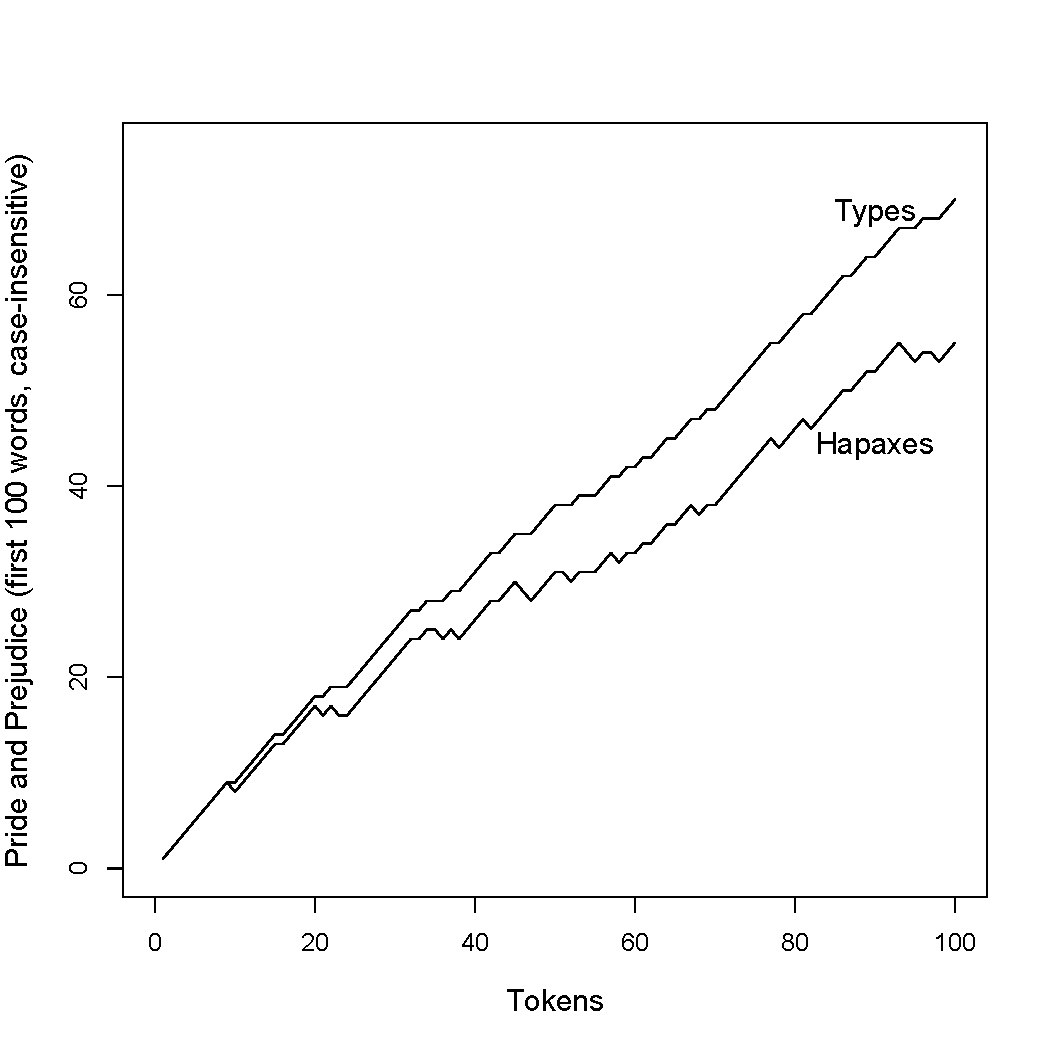
\includegraphics[width=\textwidth]{figures/prideandprejudiceonehundred}
\end{minipage}%
\begin{minipage}{.5\textwidth}
 \centering
 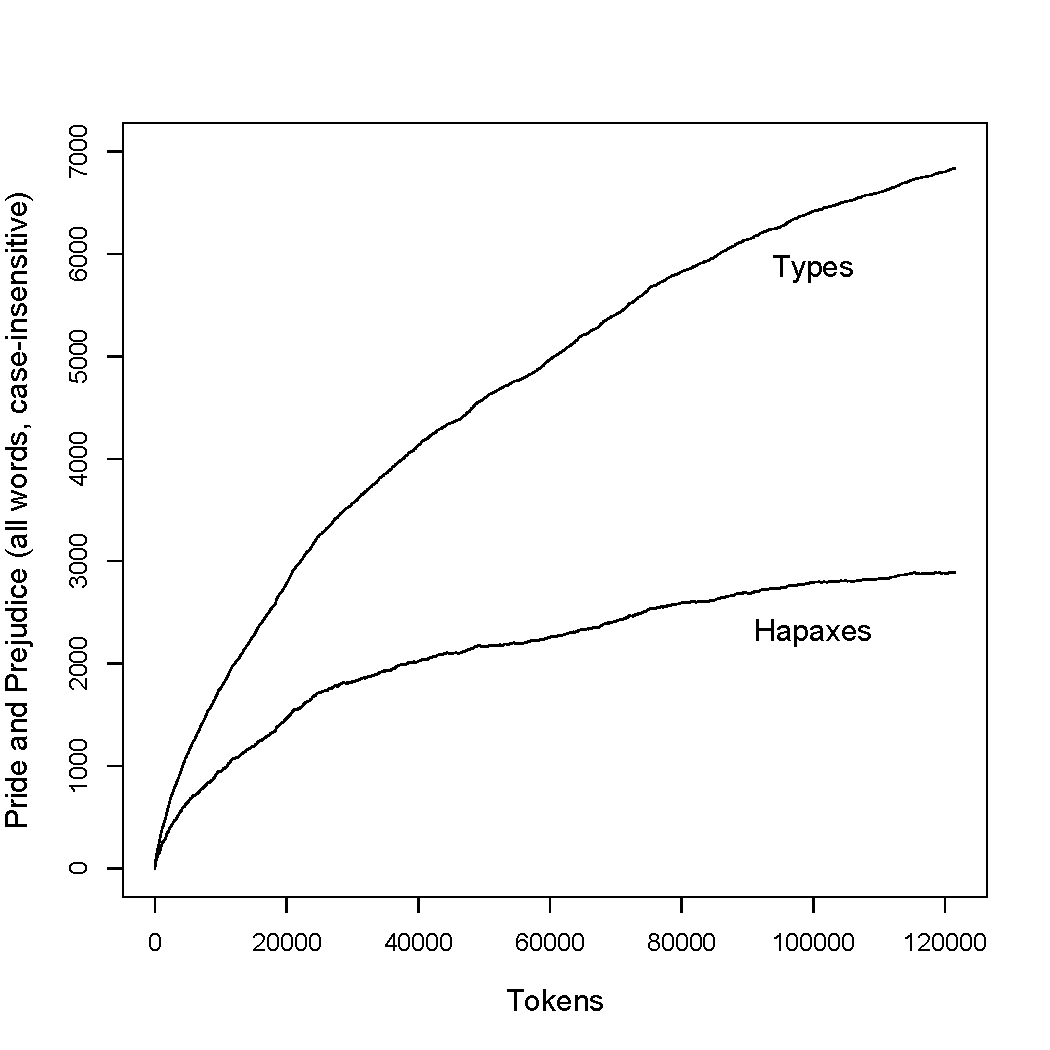
\includegraphics[width=\textwidth]{figures/prideandprejudiceall}
\end{minipage}
\end{figure}

As we can see by looking at the first 100 words, type \is{type (category)} and hapax \is{hapax legomenon} counts fall below the token counts fairly quickly: after 20 tokens, the TTR \is{type-token ratio} is $\nicefrac{18}{20} = 0.9$ and the HTR \is{hapax-token ratio} is $\nicefrac{17}{20} = 0.85$, after 40 tokens the TTR is $\nicefrac{31}{40} = 0.775$ and the HTR is $\nicefrac{26}{40} = 0.65$, after 60 tokens the HTR is $\nicefrac{42}{60} = 0.7$ and the TTR is $\nicefrac{33}{60} = 0.55$, and so on (note also how the hapax\hyp{}token \is{hapax legomenon} ratio sometimes drops before it rises again, as words that were hapaxes up to a particular point in the text reoccur and cease to be counted as hapaxes). If we zoom out and look at the entire novel, \is{literary language} we see that the growth in hapaxes slows considerably, to the extent that it has almost stopped by the time we reach the end of the novel. The growth in types \is{type (category)} also slows, although not as much as in the case of the hapaxes. \is{hapax legomenon} In both cases this means that the ratios will continue to fall as the number of tokens increases.

Now imagine we wanted to use the TTR \is{type-token ratio} and the HTR \is{hapax-token ratio} as measures of Jane Austen's overall lexical productivity \is{productivity} (referred to as ``lexical richness'' in computational stylistics \is{style} and in second\hyp{}language teaching): if we chose a small sample of her writing, the TTR and the HTR would be larger than if we chose a large \is{corpus size} sample, to the extent that the scores derived from the two samples would differ significantly. \tabref{tab:austenttr} shows what would happen if we compared the TTR of the first chapter with the TTR of the entire rest of the \is{literary language} novel.

\begin{table}
\caption{Type/token ratios in the novel \textit{Pride and Prejudice}}
\label{tab:austenttr}
\begin{tabular}[t]{llccr}
\lsptoprule
 & & \multicolumn{2}{c}{\textvv{Type}} & \\\cmidrule(lr){3-4}
 & & \textvv{new} & \textvv{$\neg$new} & Total \\
\midrule
\textvv{\makecell[lt]{Text Sample}}
	& \textvv{first chapter}
		& \makecell[t]{\num{321}\\\small{(\num{47.29})}}
		& \makecell[t]{\num{6829}\\\small{(\num{7102.71})}}
		& \makecell[t]{\num{7150}\\} \\
	& \textvv{$\neg$first chapter}
		& \makecell[t]{\num{528}\\\small{(\num{801.71})}}
		& \makecell[t]{\num{120679}\\\small{(\num{120405.29})}}
		& \makecell[t]{\num{121207}\\} \\
\midrule
	& Total
		& \makecell[t]{\num{849}}
		& \makecell[t]{\num{127508}}
		& \makecell[t]{\num{128357}} \\
\lspbottomrule
\end{tabular}
\end{table}
% me: chisq.test(matrix(c(321,528,6829,120679),ncol=2),corr=FALSE)

The TTR \is{type-token ratio} for the first chapter is an impressive 0.3781, that for the rest of the novel \is{literary language} is a measly 0.0566, and the difference is highly significant ($\chi^2 = 1688.7, \df = 1, p < 0.001, \phi = 0.1147$). \is{chi-square test} But this is not because there is anything special about the first chapter; the TTR for the second chapter is 0.3910, that for the third is 0.3457, that for chapter 4 is 0.3943, and so on. The reason why the first chapter (or any chapter) looks as though it has a significantly higher TTR than the novel \is{literary language} as a whole is simply because the TTR will drop as the size \is{corpus size} of the text increases.

Therefore, comparing TTRs \is{type-token ratio} derived from samples of different sizes \is{corpus size} will always make the smaller sample look more productive. \is{productivity} In other words, we cannot compare such TTRs, let alone evaluate the differences statistically -- the result will simply be meaningless. The same is true for HTRs, \is{hapax-token ratio} with the added problem that, under certain circumstances, it will decrease at some point as we keep increasing the sample size: \is{corpus size} at some point, all possible words will have been used, so unless new words are added to the language, the number of hapaxes \is{hapax legomenon} will shrink again and finally drop to zero when all existing types \is{type (category)} have been used at least twice.

We will encounter the same problem when we compare the TTR \is{type-token ratio} or HTR \is{hapax-token ratio} of particular affixes \is{affix} or other linguistic phenomena, rather than that of a text. Consider Figures \ref{fig:izettrhtr}a and \ref{fig:izettrhtr}b, which show the TTR and the HTR of the verb \is{verb} suffixes \is{affix} \textit{-ise/-ize} (occurring in words like \textit{realize}, \textit{maximize} or \textit{liquidize}) and \textit{-ify} (occurring in words like \textit{identify}, \textit{intensify} or \textit{liquify}).

\begin{figure}
\caption{TTRs and HTRs for \textit{-ise/-ize} and \textit{-ify} in the LOB corpus}
\label{fig:izettrhtr}
\begin{minipage}{.5\textwidth}
 \centering
 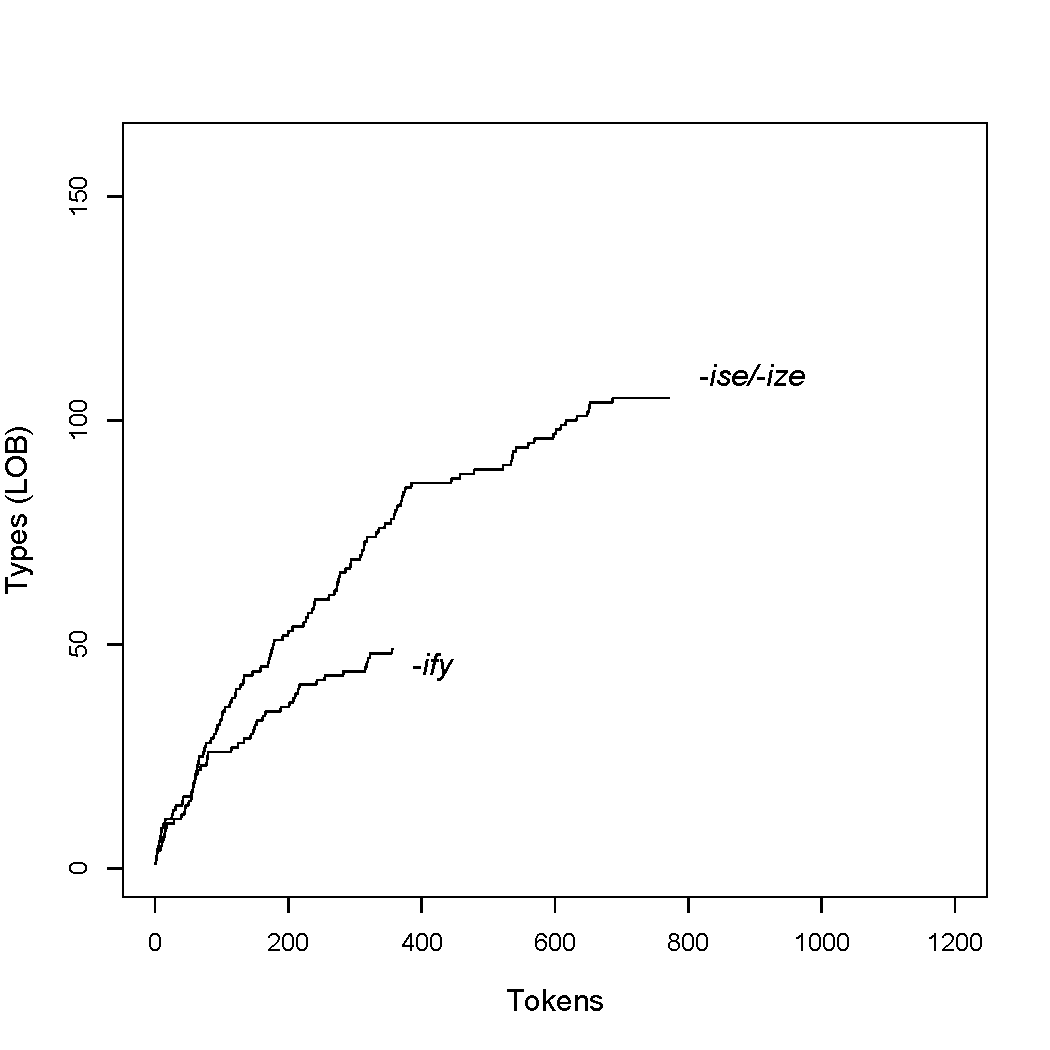
\includegraphics[width=\textwidth]{figures/lobiseifytypes}
\end{minipage}%
\begin{minipage}{.5\textwidth}
 \centering
 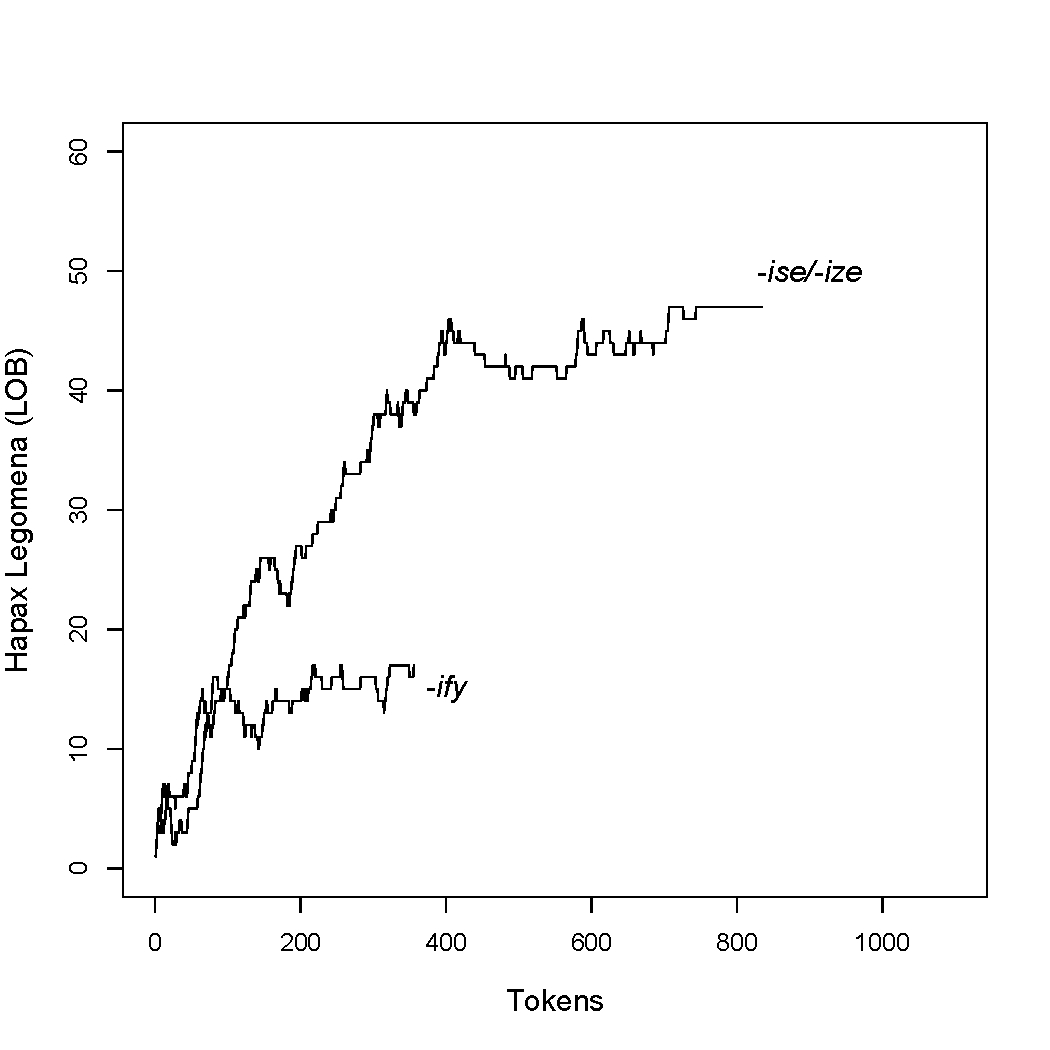
\includegraphics[width=\textwidth]{figures/lobiseifyhapaxes}
\end{minipage}
\end{figure}

As we can see, the TTR \is{type-token ratio} and HTR \is{hapax-token ratio} of both affixes \is{affix} behave roughly like that of Jane Austen's vocabulary as a whole as we increase sample size: \is{corpus size} both of them grow fairly quickly at first before their growth slows down; the latter happens more quickly in the case of the HTR than in the case of the TTR, and, again, we observe that the HTR sometimes decreases as types \is{type (category)} that were hapaxes \is{hapax legomenon} up to a particular point in the sample reoccur and cease to be hapaxes.

Taking into account the entire sample, the TTR \is{type-token ratio} for \textit{-ise/-ize} is $\nicefrac{105}{834} = 0.1259$ and that for \textit{-ify} is $\nicefrac{49}{356} = 0.1376$; it seems that \textit{-ise/-ize} is slightly more important to the lexicon \is{lexicon} of English than \textit{-ify}. A $\chi^2$ \is{chi-square test} test suggests that the difference is not significant (cf. \tabref{tab:izeifyttr}; $\chi^2 = 0.3053, \df = 1, p > 0.05$).

\begin{table}
\caption{Type/token ratios of \textit{-ise/-ize} and \textit{-ify} (LOB)}
\label{tab:izeifyttr}
\begin{tabularx}{.67\textwidth}{Qlccr}
\lsptoprule
 & & \multicolumn{2}{c}{\textvv{Type}} & \\\cmidrule(lr){3-4}
 & & \textvv{new} & \textvv{seen before} & Total \\
\midrule
\textvv{\makecell[lt]{Affix}}
	& \textvv{-ise/-ize}
		& \makecell[t]{\num{105}\\\small{(\num{107.93})}}
		& \makecell[t]{\num{729}\\\small{(\num{726.07})}}
		& \makecell[t]{\num{834}\\} \\
	& \textvv{-ify}
		& \makecell[t]{\num{49}\\\small{(\num{46.07})}}
		& \makecell[t]{\num{307}\\\small{(\num{309.93})}}
		& \makecell[t]{\num{356}\\} \\
\midrule
	& Total
		& \makecell[t]{\num{154}}
		& \makecell[t]{\num{1036}}
		& \makecell[t]{\num{1190}} \\
\lspbottomrule
\multicolumn{5}{l}{\scriptsize{Supplementary Online Material: EWTN}} \\ %OSM
\end{tabularx}
\end{table}
% me: chisq.test(matrix(c(105,49,729,307),ncol=2),corr=FALSE)

Likewise, taking into account the entire sample, the HTR \is{hapax-token ratio} for \textit{-ise/-ize} is $\nicefrac{47}{834} = 0.0563$ and that for \textit{-ify} is $\nicefrac{17}{365} = 0.0477$; it seems that \textit{-ise/-ize} is slightly more productive \is{productivity} than \textit{-ify}. However, again, the difference is not significant (cf. \tabref{tab:izeifyhtr}; $\chi^2 = 0.3628, \df = 1, p > 0.05$).

\begin{table}
\caption{Hapax/token ratios of \textit{-ise/-ize} and \textit{-ify} (LOB)}
\label{tab:izeifyhtr}
\begin{tabularx}{.67\textwidth}{Qlccr}
\lsptoprule
 & & \multicolumn{2}{c}{\textvv{Type}} & \\\cmidrule(lr){3-4}
 & & \textvv{hapax} & \textvv{$\neg$hapax} & Total \\
\midrule
\textvv{\makecell[lt]{Affix}}
	& \textvv{-ise/-ize}
		& \makecell[t]{\num{47}\\\small{(\num{44.85})}}
		& \makecell[t]{\num{787}\\\small{(\num{789.15})}}
		& \makecell[t]{\num{834}\\} \\
	& \textvv{-ify}
		& \makecell[t]{\num{17}\\\small{(\num{19.15})}}
		& \makecell[t]{\num{339}\\\small{(\num{336.85})}}
		& \makecell[t]{\num{356}\\} \\
\midrule
	& Total
		& \makecell[t]{\num{64}}
		& \makecell[t]{\num{1126}}
		& \makecell[t]{\num{1190}} \\
\lspbottomrule
\end{tabularx}
\end{table}
% me: chisq.test(matrix(c(47,17,787,339),ncol=2),corr=FALSE)

However, note that \textit{-ify} has a token \is{token (instance)} frequency \is{frequency!token} that is less than half of that of \textit{-ise/-ize}, so the sample is much smaller: as in the example of lexical richness in \textit{Pride and Prejudice}, this means that the TTR \is{type-token ratio} and the HTR \is{hapax-token ratio} of this smaller sample are exaggerated and our comparisons in Tables~\ref{tab:izeifyttr} and~\ref{tab:izeifyhtr} as well as the accompanying statistics are, in fact, completely meaningless.

The simplest way of solving the problem of different sample sizes \is{corpus size} is to create samples of equal size for the purposes of comparison. We simply take the size of the smaller of our two samples and draw a random sample of the same size from the larger of the two samples (if our data sets are large enough, it would be even better to draw random samples for both affixes). \is{affix} This means that we lose some data, but there is nothing we can do about this (note that we can still include the discarded data in a qualitative \is{qualitative research} description \is{description} of the affix \is{affix} in question).\footnote{In studies of lexical richness, a measure called \textit{Mean Segmental Type\hyp{}Token Ratio} (MSTTR) \is{type-token ratio!mean segmental} is sometimes used \citep[cf.][]{johnson_program_1944}. This measure is derived by dividing the texts under investigation into segments of equal size (often segments of 100 words), determining the TTR \is{type-token ratio} for each segment, and then calculating an average TTR. This allows us to compare the TTR of texts of different sizes without discarding any data. However, this method is not applicable to the investigation of morphological \is{morphology} productivity, \is{productivity} as most samples of 100 words (or even 1000 or \num{10000} words) will typically not contain enough cases of a given morpheme to determine a meaningful TTR.}

Figures \ref{fig:izesamplettrhtr}a and \ref{fig:izesamplettrhtr}b show the growth rates of the TTR \is{type-token ratio} and the HTR \is{hapax-token ratio} of a sub\hyp{}sample of 356 tokens of \textit{-ise/-ize} in comparison with the total sample of the same size for \textit{-ify} (the sample was derived by first deleting every second hit, \is{hit} then every seventh hit and finally every ninetieth hit, making sure that the remaining hits are spread throughout the corpus).

\begin{figure}
\caption{TTRs and HTRs for \textit{-ise/-ize} and \textit{-ify} in the LOB corpus\label{fig:izesamplettrhtr}}
\begin{minipage}{.5\textwidth}
 \centering
 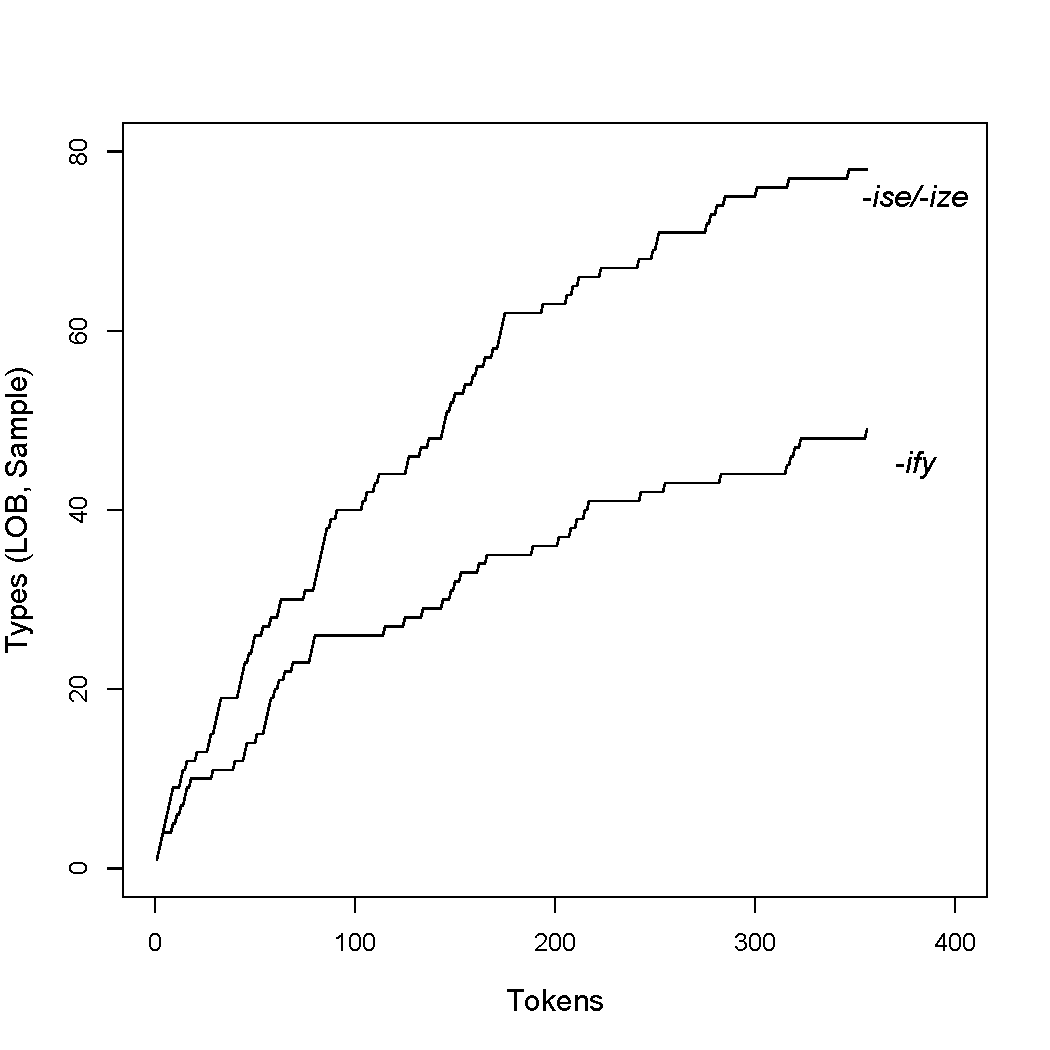
\includegraphics[width=\textwidth]{figures/lobsampleiseifytypes}
\end{minipage}%
\begin{minipage}{.5\textwidth}
 \centering
 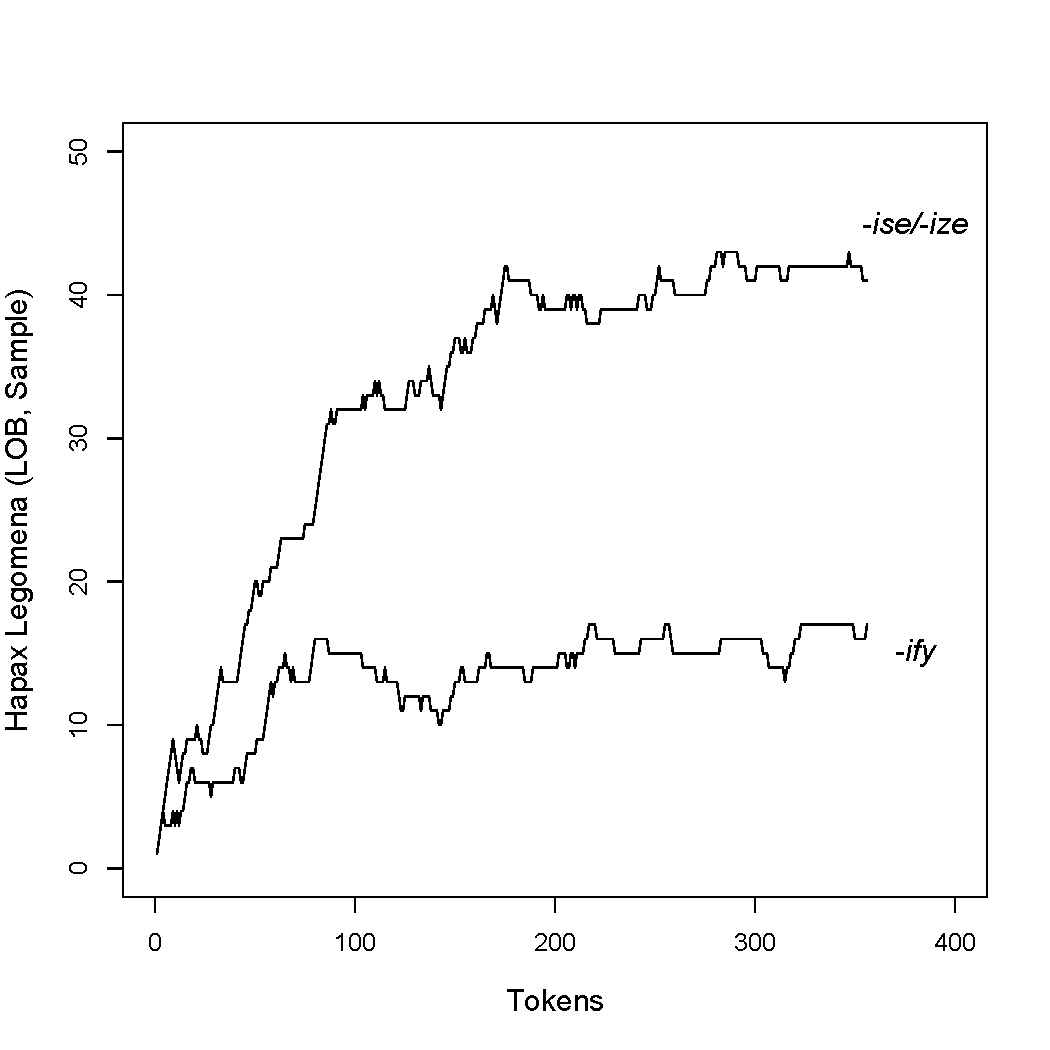
\includegraphics[width=\textwidth]{figures/lobsampleiseifyhapaxes}
\end{minipage}
\end{figure}

The TTR \is{type-token ratio} of \textit{-ise/-ize} based on the random sub\hyp{}sample is $\nicefrac{78}{356} = 0.2191$, that of \textit{-ify} is still $\nicefrac{49}{356} = 0.1376$; the difference between the two suffixes \is{affix} is much clearer now, and a $\chi^2$ test shows that it is very significant, although the effect size \is{effect size} is weak (cf. \tabref{tab:izeifyttrsample}; $\chi^2 = 8.06, \df = 1, p < 0.01, \phi = 0.1064$).

\begin{table}
\caption{Type/token ratios of \textit{-ise/-ize}/\textit{-ise/-ize} (sample) and \textit{-ify} (LOB)}
\label{tab:izeifyttrsample}
\begin{tabularx}{.67\textwidth}{Qlccr}
\lsptoprule
 & & \multicolumn{2}{c}{\textvv{Type}} & \\\cmidrule(lr){3-4}
 & & \textvv{new} & \textvv{seen before} & Total \\
\midrule
\textvv{\makecell[lt]{Affix}}
	& \textvv{-ise/-ize}
		& \makecell[t]{\num{78}\\\small{(\num{63.50})}}
		& \makecell[t]{\num{278}\\\small{(\num{292.50})}}
		& \makecell[t]{\num{356}\\} \\
	& \textvv{-ify}
		& \makecell[t]{\num{49}\\\small{(\num{63.50})}}
		& \makecell[t]{\num{307}\\\small{(\num{292.50})}}
		& \makecell[t]{\num{356}\\} \\
\midrule
	& Total
		& \makecell[t]{\num{127}}
		& \makecell[t]{\num{585}}
		& \makecell[t]{\num{712}} \\
\lspbottomrule
\end{tabularx}
\end{table}
% me: chisq.test(matrix(c(78,49,278,307),ncol=2),corr=FALSE)

Likewise, the HTR \is{hapax-token ratio} of \textit{-ise/-ize} based on our sub\hyp{}sample is $\nicefrac{41}{356} = 0.1152$, the HTR of \textit{-ify} remains $\nicefrac{17}{365} = 0.0477$. Again, the difference is much clearer, and it, too, is now very significant, again with a weak effect size \is{effect size} (cf. \tabref{tab:izeifyhtrsample}; $\chi^2 = 10.81, \df = 1, p < 0.01, \phi =  0.1232$).\is{chi-square test}

\begin{table}
\caption{Hapax/token ratios of \textit{-ise/-ize} (sample) and \textit{-ify} (LOB)}
\label{tab:izeifyhtrsample}
\begin{tabularx}{.67\textwidth}{Qlccr}
\lsptoprule
 & & \multicolumn{2}{c}{\textvv{Type}} & \\\cmidrule(lr){3-4}
 & & \textvv{hapax} & \textvv{$\neg$hapax} & Total \\
\midrule
\textvv{\makecell[lt]{Affix}}
	& \textvv{-ise/-ize}
		& \makecell[t]{\num{41}\\\small{(\num{29.00})}}
		& \makecell[t]{\num{315}\\\small{(\num{327.00})}}
		& \makecell[t]{\num{356}\\} \\
	& \textvv{-ify}
		& \makecell[t]{\num{17}\\\small{(\num{29.00})}}
		& \makecell[t]{\num{339}\\\small{(\num{327.00})}}
		& \makecell[t]{\num{356}\\} \\
\midrule
	& Total
		& \makecell[t]{\num{58}}
		& \makecell[t]{\num{654}}
		& \makecell[t]{\num{712}} \\
\lspbottomrule
\end{tabularx}
\end{table}
% me: chisq.test(matrix(c(41,17,315,339),ncol=2),corr=FALSE)

In the case of the HTR, \is{hapax-token ratio} decreasing the sample size \is{corpus size} is slightly more problematic than in the case of the TTR. \is{type-token ratio} The proportion of hapax \is{hapax legomenon} legomena actually resulting from productive \is{productivity} rule application becomes smaller as sample size decreases. Take example (\ref{ex:shakspearecinna}) from Shakespeare's \textit{Julius Caesar} above: the words \textit{directly}, \textit{briefly} and \textit{truly} are all hapaxes \is{hapax legomenon} in the passage cited, but they are clearly not the result of a productively \is{productivity} applied rule\hyp{}application (all of them have their own entries in the OALD, for example). As we increase the sample, they cease to be hapaxes (\textit{directly} occurs 9 times in the entire play, \textit{briefly} occurs 4 times and \textit{truly} 8 times). This means that while we must draw random samples of equal size \is{corpus size} in order to compare HTRs, \is{hapax-token ratio} we should make sure that these samples are as large as possible.

\section{Case studies}
\label{sec:moprphologycasestudies}

\subsection{Morphemes and stems}
\label{sec:morphemesandstems}

One general question in (derivational) morphology \is{morphology} concerns the category of the stem \is{stem} which an affix \is{affix} may be attached to. This is obviously a descriptive \is{description} issue that can be investigated on the basis of corpora very straightforwardly simply by identifying all types \is{type (category)} containing the affix \is{affix} in question and describing their internal structure. In the case of affixes \is{affix} with low productivity, \is{productivity} this will typically add little insight over studies based on dictionaries, \is{dictionary} but for productive affixes, \is{affix} a corpus analysis will yield more detailed and comprehensive results since corpora will contain spontaneously produced or at least recently created items not (yet) found in dictionaries. \is{dictionary} Such newly created words will often offer particularly clear insights into constraints that an affix \is{affix} places on its stems. \is{statistics} Finally, corpus\hyp{}based approaches are without an alternative in diachronic \is{diachrony} studies and yield particularly interesting results when used to study changes in the quality or degree of productivity, \is{productivity} (cf. for example \citealt{dalton-puffer_french_1996}).

In the study of constraints placed by derivational affixes \is{affix} on the stems \is{stem} that they combine with, the combinability of derivational morphemes \is{morphology} (in an absolute sense or in terms of preferences) is of particular interest. Again, corpus linguistics is a uniquely useful tool to investigate this.

Finally, there are cases where two derivational morphemes \is{morphology} are in direct competition because they are functionally roughly equivalent (e.g. \textit{-ness} and \textit{-ity}, both of which form abstract nouns \is{noun} from typically adjectival \is{adjective} bases, \textit{-ise/-ize} and \textit{-ify}, which form process \is{aktionsart} verbs \is{verb} from nominal \is{noun} and adjectival \is{adjective} bases, or \textit{-ic} and \textit{-ical}, which form adjectives \is{adjective} from typically nominal bases). Here, too, corpus linguistics provides useful tools, for example to determine whether the choice between affixes \is{affix} is influenced by syntactic, \is{syntax} semantic or phonological properties of \is{stem} stems.

\subsubsection{Case study: Phonological constraints on \textit{-ify}}
\label{sec:phonologicalconstraintsofify}

As part of a larger argument that \textit{-ise/-ize} and \textit{-ify} should be considered phonologically conditioned allomorphs, \citet{plag_morphological_1999} investigates the phonological constraints that \textit{-ify} places on its stems. \is{statistics} First, he summarizes the properties of stems in established words with \textit{-ify} as observed in the literature. Second, he checks these observations against a sample of twenty\hyp{}three recent (20th century) coinages from a corpus of neologisms \is{neologism} to ensure that the constraints also apply to productive \is{productivity} uses of the affix. \is{affix} This is a reasonable approach. The affix \is{affix} was first borrowed into English as part of a large number of French loanwords beginning in the late 13th century; two thirds of all non\hyp{}hapax \is{hapax legomenon} types \is{type (category)} and 19 of the 20 most frequent types found in the BNC \is{BNC} are older than the 19th century. Thus, it is possible that the constraints observed in the literature are historical remnants not relevant to new coinages.

The most obvious constraint is that the syllable \is{syllable} directly preceding \textit{-ify} must carry the main stress of the word. This has a number of consequences, of which we will focus on two: First, monosyllabic stems \is{stem} (as in \textit{falsify}) are preferred, since they always meet this criterion. Second, if a polysyllabic stem ends in an unstressed syllable, the stress must be shifted to that syllable (as in \textit{perSONify} from \textit{PERson});\footnote{This is a simplification: stress\hyp{}shift only occurs with unstressed closed syllables or sequence of two unstressed syllables \is{syllable} (\textit{SYLlable} -- \textit{sylLAbify}). Occasionally, stem\hyp{}final \is{statistics} consonants \is{consonant} are deleted (as in \textit{liquid} -- \textit{liquify}); cf. \citet{plag_morphological_1999} for a more detailed discussion.} since this reduces the transparency of the stem, there should be a preference for those polysyllabic stems \is{stem} which already have the stress on the final \is{syllable} syllable.

Plag simply checks his neologisms \is{neologism} against the literature, but we will evaluate the claims from the literature quantitatively. \is{quantitative research} Our main hypothesis will be that neologisms with \textit{-ify} do not differ from established types \is{type (category)} with respect to the fact that the syllable \is{syllable} directly preceding the suffix \is{affix} must carry primary stress, with the consequences that (i) they prefer monosyllabic stems, \is{statistics} and (ii) if the stem \is{stem} is polysyllabic, they prefer stems that already have the primary stress on the last syllable. Our independent variable is therefore \textsc{Lexical Status} with the values \textsc{established word} vs. \textsc{neologism} \is{neologism} (which will be operationalized \is{operationalization} presently). Our dependent variables are \textsc{Syllabicity} \is{syllable} with the values \textsc{monosyllabic} and \textsc{polysyllabic}, and \textsc{Stress Shift} with the values \textsc{required} vs. \textsc{not required} (both of which should be self\hyp{}explanatory).

Our design \is{research design} compares two predefined groups of types \is{type (category)} with respect to the distribution \is{distribution!conditional} that particular properties have in these groups; this means that we do not need to calculate TTRs \is{type-token ratio} or HTRs, \is{hapax-token ratio} but that we need operational \is{operationalization} definitions of the values \textsc{established word} and \textsc{neologism}. \is{neologism} Following Plag, let us define \textsc{neologism} as ``coined in the 20th century'', but let us use a large historical dictionary \is{dictionary} (the Oxford English Dictionary, \is{OED} 3rd edition) and a large \is{corpus size} corpus (the BNC) \is{BNC} in order to identify words matching this definition; this will give us the opportunity to evaluate the idea that hapax \is{hapax legomenon} legomena are a good way of operationalizing \is{productivity} productivity.

Excluding cases with prefixed \is{affix} stems, \is{statistics} the OED \is{OED} contains 456 entries or sub\hyp{}entries for verbs \is{verb} with \textit{-ify}, 31 of which are first documented in the 20th century. Of the latter, 21 do not occur in the BNC \is{BNC} at all, and 10 do occur in the BNC, but are not hapaxes \is{hapax legomenon} (see \tabref{tab:ifyneologisms} below). The BNC contains 30 hapaxes, of which 13 are spelling errors and 7 are first documented in the OED \is{OED} before the 20th century (\textit{carbonify}, \textit{churchify}, \textit{hornify}, \textit{preachify}, \textit{saponify}, \textit{solemnify}, \textit{townify}). This leaves 10 hapaxes that are plausibly regarded as neologisms, \is{neologism} none of which are listed in the OED \is{OED} (again, see \tabref{tab:ifyneologisms}). In addition, there are four types \is{type (category)} in the BNC \is{BNC} that are not hapax \is{hapax legomenon} legomena, but that are not listed in the OED; \is{OED} careful cross\hyp{}checks show that these are also neologisms. Combining all sources, this gives us 45 neologisms.

\begin{table}
\caption{Twentieth century neologisms with \textit{-ify}}
\label{tab:ifyneologisms}
\begin{tabular}[t]{ll}
\lsptoprule
\multicolumn{2}{l}{First documented in the OED in the 20th century} \\\midrule
(i) & also occur in the BNC, but not as hapaxes: \\
 & \makecell[tl]{\textit{bourgeoisify}, \textit{esterify}, \textit{gentrify}, \textit{karstify}, \textit{massify}, \textit{Nazify}, \textit{syllabify}, \\ \textit{vinify}, \textit{yuppify}, \textit{zombify}} \\
(ii) & do not occur in the BNC: \\
 & \makecell[tl]{\textit{ammonify}, \textit{aridify}, \textit{electronify}, \textit{glassify}, \textit{humify}, \textit{iconify}, \textit{jazzify}, \\ \textit{mattify}, \textit{metrify}, \textit{mucify}, \textit{nannify}, \textit{passivify}, \textit{plastify}, \textit{probabilify}, \\\textit{Prussify}, \textit{rancidify}, \textit{sinify}, \textit{trendify}, \textit{trustify}, \textit{tubify}, \textit{youthify}} \\
\midrule\multicolumn{2}{l}{Not documented in the OED at all} \\\midrule
(iii) & occur in the BNC as hapaxes: \\
 & \makecell[tl]{\textit{faintify}, \textit{fuzzify}, \textit{lewisify}, \textit{rawify}, \textit{rockify}, \textit{sickify}, \textit{sonify}, \textit{validify}, \\ \textit{yankify}, \textit{yukkify}} \\
(iv) & occur in the BNC, but not as hapaxes: \\
 & \makecell[tl]{\textit{commodify}, \textit{desertify}, \textit{extensify}, \textit{geriatrify}} \\
\lspbottomrule
\end{tabular}
\end{table}

Before we turn to the definition and sampling of established types, \is{type (category)} let us determine the precision \is{precision} and recall \is{recall} of the operational \is{operationalization} definition of neologism \is{neologism} as ``hapax \is{hapax legomenon} legomenon in the BNC'', \is{BNC} using the formulas introduced in \chapref{ch:retrievalannotation}. Precision is defined as the number of true positives (items that were found and that actually are what they are supposed to be) divided by the number of all positives (all items found); 10 of the 30 hapaxes in the BNC \is{BNC} are actually neologisms, so the precision is $\nicefrac{10}{30} = 0.3333$. Recall is defined as the number of true positives divided by the number of true positives and false negatives (i.e. all items that should have been found); 10 of the 45 neologisms \is{neologism} were actually found by using the hapax definition, so the recall is $\nicefrac{10}{45} = 0.2222$. In other words, neither precision \is{precision} nor recall of the method are very good, at least for moderately productive \is{productivity} affixes \is{affix} like \textit{-ify} (the method will presumably give better results with highly productive affixes). \is{affix} Let us also determine the recall of neologisms from the OED \is{OED} (using the definition ``first documented in the 20th century according to the OED''): the OED \is{OED} lists 31 of the 45 neologisms, \is{neologism} so the recall is $\nicefrac{31}{45} = 0.6889$; this is much better than the recall \is{recall} of the corpus\hyp{}based hapax \is{hapax legomenon} definition, but it also shows that if we combine corpus data and dictionary \is{dictionary} data, we can increase coverage substantially even for moderately productive affixes.\is{productivity}\is{affix}

Let us now turn to the definition of \textsc{established types}. \is{type (category)} Given our definition of \textsc{neologisms}, \is{neologism} established types would first have to be documented before the 20th century, so we could use the 420 types in the OED \is{OED} that meet this criterion (again, excluding prefixed \is{affix} forms). However, these 420 types contain many very rare or even obsolete forms, like \textit{duplify} `to make double', \textit{eaglify} `to make into an eagle' or \textit{naucify} `to hold in low esteem'. Clearly, these are not ``established'' in any meaningful sense, so let us add the requirement that a type must occur in the BNC \is{BNC} at least twice to count as established. Let us further limit the category to verbs \is{verb} first documented before the 19th century, in order to leave a clear diachronic \is{diachrony} gap between the established types \is{type (category)} and the productive \is{productivity} types. This leaves the words in \tabref{tab:ifycontrol}.\footnote{Interestingly, leaving out words coined in the 19th century does not make much of a difference: although the 19th century saw a large number of coinages (with 138 new types \is{type (category)} it was the most productive \is{productivity} century in the history of the suffix), \is{affix} few of these are frequent enough today to occur in the BNC; \is{BNC} if anything, we should actually extend our definition of neologisms \is{neologism} to include the 19th century.}

\begin{table}
\caption{Control sample of established types with the suffix \textit{-ify}.}
\label{tab:ifycontrol}
\begin{tabular}[t]{l}
\lsptoprule
\makecell[tl]{
\textit{acidify}, \textit{amplify}, \textit{beatify}, \textit{beautify}, \textit{certify}, \textit{clarify}, \textit{classify}, \\ \textit{crucify}, \textit{damnify}, \textit{deify}, \textit{dignify}, \textit{diversify}, \textit{edify}, \textit{electrify}, \\ \textit{exemplify}, \textit{falsify}, \textit{fortify}, \textit{Frenchify}, \textit{fructify}, \textit{glorify}, \textit{gratify}, \\ \textit{identify}, \textit{indemnify}, \textit{justify}, \textit{liquify}\slash \textit{liquefy}, \textit{magnify}, \textit{modify}, \\ \textit{mollify}, \textit{mortify}, \textit{mummify}, \textit{notify}, \textit{nullify}, \textit{ossify}, \textit{pacify}, \\ \textit{personify}, \textit{petrify}, \textit{prettify}, \textit{purify}, \textit{qualify}, \textit{quantify}, \textit{ramify}, \\ \textit{rarify}, \textit{ratify}, \textit{rectify}, \textit{sacrify}, \textit{sanctify}, \textit{satisfy}, \textit{scarify}, \\ \textit{signify}, \textit{simplify}, \textit{solidify}, \textit{specify}, \textit{stratify}, \textit{stultify}, \textit{terrify}, \\ \textit{testify}, \textit{transmogrify}, \textit{typify}, \textit{uglify}, \textit{unify}, \textit{verify}, \textit{versify}, \\ \textit{vilify}, \textit{vitrify}, \textit{vivify}} \\
\lspbottomrule
\end{tabular}
\end{table}

Let us now evaluate the hypotheses. \tabref{tab:ifysyllabicity} shows the type \is{type (category)} frequencies \is{frequency!type} for monosyllabic \is{syllable} and polysyllabic stems \is{stem} in the two samples. In both cases, there is a preference for monosyllabic stems (as expected), \is{frequency!expected} but interestingly, this preference is less strong among the neologisms \is{neologism} than among the established types and this difference is very significant ($\chi^2 = 7.37, \df = 1, p < 0.01, \phi = 0.2577$).

\begin{table}
\caption{Monosyllabic and bisyllabic stems with \textit{-ify}}
\label{tab:ifysyllabicity}
\begin{tabular}[t]{llccr}
\lsptoprule
 & & \multicolumn{2}{c}{\textvv{Number of Syllables}} & \\\cmidrule(lr){3-4}
 & & \textvv{monosyllabic} & \textvv{polysyllabic} & Total \\
\midrule
\textvv{\makecell[lt]{Status}}
	& \textvv{established}
		& \makecell[t]{\num{57}\\\small{(\num{51.14})}}
		& \makecell[t]{\num{9}\\\small{(\num{14.86})}}
		& \makecell[t]{\num{66}\\} \\
	& \textvv{neologism}
		& \makecell[t]{\num{29}\\\small{(\num{34.86})}}
		& \makecell[t]{\num{16}\\\small{(\num{10.14})}}
		& \makecell[t]{\num{45}\\} \\
\midrule
	& Total
		& \makecell[t]{\num{86}}
		& \makecell[t]{\num{25}}
		& \makecell[t]{\num{111}} \\
\lspbottomrule
\end{tabular}
\end{table}
% me: chisq.test(matrix(c(57,29,9,16),ncol=2),corr=FALSE)

Given the fact that there is a significantly higher number of neologisms \is{neologism} with polysyllabic \is{syllable} stems \is{stem} than expected \is{frequency!expected} on the basis of established types, \is{type (category)} the second hypothesis becomes more interesting: does this higher number of polysyllabic \is{syllable} stems \is{stem} correspond with a greater willingness to apply it to stems that then have to undergo stress shift (which would be contrary to our hypothesis, which assumes that there will be no difference between established types and \is{neologism} neologisms)?

\tabref{tab:ifystressshift} shows the relevant data: it seems that there might indeed be such a greater willingness, as the number of neologisms \is{neologism} with polysyllabic \is{syllable} stems \is{stem} requiring stress shift is higher than expected; \is{frequency!expected} however, the difference is not statistically significant ($\chi^2 = 1.96, \df = 1, p > 0.05, \phi = 0.28$) (strictly speaking, we cannot use the $\chi^2$ \is{chi-square test} test here, since half of the expected frequencies are below 5, but Fisher's exact test \is{Fisher's exact test} confirms that the difference is not significant).

\begin{table}
\caption{Stress shift with polysyllabic stems with \textit{-ify}}
\label{tab:ifystressshift}
\begin{tabular}[t]{llccr}
\lsptoprule
 & & \multicolumn{2}{c}{\textvv{Shift}} & \\\cmidrule(lr){3-4}
 & & \textvv{not required} & \textvv{required} & Total \\
\midrule
\textvv{\makecell[lt]{Status}}
	& \textvv{established}
		& \makecell[t]{\num{3}\\\small{(\num{4.68})}}
		& \makecell[t]{\num{6}\\\small{(\num{4.32})}}
		& \makecell[t]{\num{9}\\} \\
	& \textvv{neologism}
		& \makecell[t]{\num{10}\\\small{(\num{8.32})}}
		& \makecell[t]{\num{6}\\\small{(\num{7.68})}}
		& \makecell[t]{\num{16}\\} \\
\midrule
	& Total
		& \makecell[t]{\num{13}}
		& \makecell[t]{\num{12}}
		& \makecell[t]{\num{25}} \\
\lspbottomrule
\end{tabular}
\end{table}
% me: chisq.test(matrix(c(3,10,6,6),ncol=2),corr=FALSE)

This case study demonstrates some of the problems and advantages of using corpora to identify neologisms \is{neologism} in addition to existing dictionaries. \is{dictionary} It also constitutes an example of a purely type\hyp{}based \is{type (category)} research design; \is{research design} note, again, that such a design is possible here because we are not interested in the type frequency \is{frequency!type} of a particular affix \is{affix} under different conditions (in which case we would have to calculate a TTR \is{type-token ratio} to adjust for different sample sizes), \is{corpus size} but in the distribution \is{distribution!conditional} of the variables \textsc{Syllable Length} \is{syllable}\is{length} and \textsc{Stress Shift} in two qualitatively different categories of types. \is{type (category)} Finally, note that the study comes to different conclusions than the impressionistic analysis in \citet{plag_morphological_1999}, so it demonstrates the advantages of strictly quantified designs.

\subsubsection{Case study: Semantic differences between \textit{-ic} and \textit{-ical}}
\label{sec:semanticdifferencesbetweenicandical}

Affixes, like words, can be related to other affixes \is{affix} by lexical relations like synonymy, \is{synonymy} antonymy, \is{antonymy} etc. In the case of (roughly) synonymous affixes, \is{affix} an obvious research question is what determines the choice between them -- for example, whether there are more fine\hyp{}grained semantic \is{semantics} differences that are not immediately apparent.

One way of approaching this question is to focus on stems \is{stem} that occur with both affixes \is{affix} (such as \textit{liqui(d)} in \textit{liquidize} and \textit{liquify}\slash \textit{liquefy}, \textit{scarce} in \textit{scarceness} and \textit{scarcity} or \textit{electr-} in \textit{electric} and \textit{electrical}) and to investigate the semantic \is{semantics} contexts in which they occur -- for example, by categorizing \is{categorization} their collocates, \is{collocation} analogous to the way \citet{taylor_near_2003} categorizes collocates of \textit{high} and \textit{tall} (cf. \chapref{ch:collocation}, Section~\ref{sec:nearsynonyms}).

A good example of this approach is found in \citet{kaunisto_electric/electrical_1999}, who investigates the pairs \textit{electric}\slash \textit{electrical} and \textit{classic}\slash \textit{classical} on the basis of the British Newspaper \is{newspaper language} \textit{Daily Telegraph}. Since his corpus is not accessible, let us use the LOB \is{LOB} corpus instead to replicate \is{replicability} his study for \textit{electric}\slash \textit{electrical}. It is a study with two nominal \is{nominal data} variables: \textsc{Affix Variant} (with the values \textsc{-ic} and \textsc{-ical}), and \textsc{Semantic Category} (with a set of values to be discussed presently). Note that this design \is{research design} can be based straightforwardly on token \is{token (instance)} frequency, \is{frequency!token} as we are not concerned with the relationship between the stem \is{stem} and the affix, \is{affix} but with the relationship between the stem\hyp{}affix combination and the nouns \is{noun} modified by it. Put differently, we are not using the token \is{token (instance)} frequency of a stem\hyp{}affix combination, but of the collocates \is{collocation} of words derived by a particular \is{affix} affix.

Kaunisto uses a mixture of dictionaries \is{dictionary} and existing literature to identify potentially interesting values for the variable \textsc{Semantic Category}; we will restrict ourselves to dictionaries here. Consider the definitions from six major dictionaries \is{dictionary} in (\ref{ex:definitionelectric}) and (\ref{ex:definitionelectrical}):

\begin{exe}
\ex \textit{electric}
\begin{xlist}
\label{ex:definitionelectric}
\ex connected with electricity; using, produced by or producing electricity (OALD)
\ex of or relating to electricity; operated by electricity (MW)
\ex working by electricity; used for carrying electricity; relating to electricity (MD)
\ex of, produced by, or worked by electricity (CALD)
\ex needing electricity to work, produced by electricity, or used for carrying electricity (LDCE)
\ex work$[$ing$]$ by means of electricity; produced by electricity; designed to carry electricity; refer$[$ring$]$ to the supply of electricity (Cobuild)
\end{xlist}

\ex \textit{electrical}
\begin{xlist}
\label{ex:definitionelectrical}
\ex connected with electricity; using or producing electricity (OALD)
\ex of or relating to electricity; operated by electricity (MW) $[$mentioned as a synonym under corresp. sense of \textit{electric}$]$
\ex working by electricity; relating to electricity (MD)
\ex related to electricity (CALD, LDCE)
\ex work[ing] by means of electricity; supply[ing] or us[ing] electricity; energy ... in the form of electricity; involved in the production and supply of electricity or electrical goods (Cobuild)
\end{xlist}
\end{exe}

MW treats the two words as largely synonymous \is{synonymy} and OALD distinguishes them only insofar as mentioning for \textit{electric}, but not \textit{electrical}, that it may refer to phenomena `produced by electricity' (this is meant to cover cases like \textit{electric current\slash charge}); however, since both words are also defined as referring to anything `connected with electricity', this is not much of a differentiation (the entry for \textit{electrical} also mentions \textit{electrical power\slash energy}). Macmillan's dictionary \is{dictionary} also treats them as largely synonymous, \is{synonymy} although it is pointed out specifically that \textit{electric} refers to entities `carrying electricity' (citing \textit{electric outlet\slash plug\slash cord}). CALD and LDCE present \textit{electrical} as a more general word for anything `related to electricity', whereas they mention specifically that \textit{electric} is used for things `worked by electricity' (e.g. \textit{electric light\slash appliance}) or `carrying electricity' (presumably \textit{cords}, \textit{outlets}, etc.) and phenomena produced by electricity (presumably \textit{current}, \textit{charge}, etc.). Collins presents both words as referring to electric(al) appliances, with \textit{electric} additionally referring to things `produced by electricity', `designed to carry electricity' or being related to the `supply of electricity' and \textit{electrical} additionally referring to `energy' or entities `involved in the production and supply of electricity' (presumably energy companies, engineers, etc.).

Summarizing, we can posit the following four broad values for our variable \textsc{Semantic Category}, with definitions that are hopefully specific enough to serve as an annotation \is{annotation} scheme:

\begin{itemize}

\item \textsc{devices} and appliances working by electricity (\textit{light}, \textit{appliance}, etc.)

\item \textsc{energy} in the form of electricity (\textit{power}, \textit{current}, \textit{charge}, \textit{energy}, etc.)

\item the \textsc{industry} researching, producing or supplying energy, i.e. companies and the people working there (\textit{company}, \textit{engineer}, etc.)

\item \textsc{circuits}, broadly defined as entities producing or carrying electricity, including (\textit{cord}, \textit{outlet}, \textit{plug}, but also \textit{power plant}, etc.)

\end{itemize}

The definitions are too heterogeneous to base a specific hypothesis on them, but we might broadly expect \textit{electric} to be more typical for the categories \textvv{device} and \textvv{circuit} and \textit{electrical} for the category \textvv{industry}.

\tabref{tab:electricalentitieslob} shows the token \is{token (instance)} frequency \is{frequency!token} with which nouns \is{noun} from these categories are referred to as \textit{electric} or \textit{electrical} in the LOB \is{LOB} corpus; in order to understand how these nouns were categorized, \is{categorization} it also lists all types \is{type (category)} found for each category (one example was discarded because it was  \is{figurative language}\is{metaphor} metaphorical).

\begin{table}
\caption{Entities described as \textit{electric} or \textit{electrical} in the LOB corpus}
\label{tab:electricalentitieslob}
\resizebox{0.9\textwidth}{!}{%
\begin{tabular}[t]{lccr}
\lsptoprule
 & \multicolumn{2}{c}{\textvv{Adjective}} & \\\cmidrule(lr){2-3}
\textvv{Noun} & \textvv{electric} & \textvv{electrical} & Total \\
\midrule
\textvv{\makecell[tl]{device}}
	& \makecell[t]{\begin{tabular}[t]{lS[table-format=2.2]}
		\small{\textit{Obs.:}} & 17 \\
		\small{\textit{Exp.:}} & 12.077922 \\
		\small{\textit{$\chi^2$:}} & 2.005879 \\
		\multicolumn{2}{l}{
			\begin{minipage}[t]{0.3\textwidth} \raggedright
			\footnotesize{\textit{bulb}, \textit{calculating machine}, \textit{chair}, \textit{cooker}, \textit{dog}, \textit{drill}, \textit{fence}, \textit{fire}, \textit{heating element}, \textit{light switch}, \textit{motor}, \textit{mowing}, \textit{stove}, \textit{torch}, \textit{tricycle}}
			\end{minipage}}
		\end{tabular}}
	& \makecell[t]{\begin{tabular}[t]{lS[table-format=2.2]}
		\small{\textit{Obs.:}} & 13 \\
		\small{\textit{Exp.:}} & 17.922078 \\
		\small{\textit{$\chi^2$:}} & 1.351788 \\
		\multicolumn{2}{l}{
			\begin{minipage}[t]{0.3\textwidth} \raggedright
			\footnotesize{\textit{amplifier}, \textit{apparatus}, \textit{fire}, \textit{goods}, \textit{machine}, \textit{machinery}, \textit{power unit}, \textit{sign}, \textit{supply}, \textit{system}, \textit{system}, \textit{transmission}}
		\end{minipage}}
		\end{tabular}}
	& 30 \\[3.1cm]
\textvv{\makecell[tl]{energy}}
	& \makecell[t]{\begin{tabular}[t]{lS[table-format=2.2]}
		\small{\textit{Obs.:}} & 11 \\
		\small{\textit{Exp.:}} & 9.662338 \\
		\small{\textit{$\chi^2$:}} & 0.185187 \\
		\multicolumn{2}{l}{
			\begin{minipage}[t]{0.3\textwidth} \raggedright
			\footnotesize{\textit{attraction}, \textit{bill}, \textit{blue}, \textit{current}, \textit{effect}, \textit{field}, \textit{force}, \textit{light}, \textit{space constant}}
			\end{minipage}}
		\end{tabular}}
	& \makecell[t]{\begin{tabular}[t]{lS[table-format=2.2]}
		\small{\textit{Obs.:}} & 13 \\
		\small{\textit{Exp.:}} & 14.337662 \\
		\small{\textit{$\chi^2$:}} & 0.124800 \\
		\multicolumn{2}{l}{
			\begin{minipage}[t]{0.3\textwidth} \raggedright
			\footnotesize{\textit{accident}, \textit{activity}, \textit{condition}, \textit{load}, \textit{output}, \textit{phenomenon}, \textit{property}, \textit{resistance}}
			\end{minipage}}
		\end{tabular}}
	& 24 \\[2.4cm]
\textvv{\makecell[tl]{circuit}}
	& \makecell[t]{\begin{tabular}[t]{lS[table-format=2.2]}
		\small{\textit{Obs.:}} & 2 \\
		\small{\textit{Exp.:}} & 2.012987 \\
		\small{\textit{$\chi^2$:}} & 0.00000008 \\
		\multicolumn{2}{l}{
			\begin{minipage}[t]{0.3\textwidth} \raggedright
			\footnotesize{\textit{battery}, \textit{line}}
			\end{minipage}}
		\end{tabular}}
	& \makecell[t]{\begin{tabular}[t]{lS[table-format=2.2]}
		\small{\textit{Obs.:}} & 3 \\
		\small{\textit{Exp.:}} & 2.987013 \\
		\small{\textit{$\chi^2$:}} & 0.564652 \\
		\multicolumn{2}{l}{
			\begin{minipage}[t]{0.3\textwidth} \raggedright
			\footnotesize{\textit{circuit}, \textit{conductivity}}
			\end{minipage}}
		\end{tabular}}
	& 5 \\[1.6cm]
\textvv{\makecell[tl]{industry}}
	& \makecell[t]{\begin{tabular}[t]{lS[table-format=2.2]}
		\small{\textit{Obs.:}} & 1 \\
		\small{\textit{Exp.:}} & 7.246753 \\
		\small{\textit{$\chi^2$:}} & 5.384746 \\
		\multicolumn{2}{l}{
			\begin{minipage}[t]{0.3\textwidth} \raggedright
			\footnotesize{\textit{company}}
			\end{minipage}}
		\end{tabular}}
	& \makecell[t]{\begin{tabular}[t]{lS[table-format=2.2]}
		\small{\textit{Obs.:}} & 17 \\
		\small{\textit{Exp.:}} & 10.753247 \\
		\small{\textit{$\chi^2$:}} & 3.628851 \\
		\multicolumn{2}{l}{
			\begin{minipage}[t]{0.3\textwidth} \raggedright
			\footnotesize{\textit{communication theory}, \textit{counterpart}, \textit{development}, \textit{engineer}, \textit{industry}, \textit{trade}, \textit{work}}
			\end{minipage}}
		\end{tabular}}
	& 18 \\[2.8cm]
\midrule
Total
	& \makecell[t]{31}
	& \makecell[t]{46}
	& \makecell[t]{77} \\
\lspbottomrule
\multicolumn{4}{l}{\scriptsize{Supplementary Online Material: KVCF}} \\ %OSM
\end{tabular}}
\end{table}
% me: query: LOB_LEGACY; [word="electric(al)?"%c][pos="N.*"]

The difference between \textit{electric} and \textit{electrical} is significant overall ($\chi^2 = 12.68$, $\df = 3, p < 0.01, \phi = 0.2869$), suggesting that the two words somehow differ with respect to their preferences for these categories. Since we are interested in the nature of this difference, it is much more insightful to look at the $\chi^2$ \is{chi-square test} components individually. This gives us a better idea where the overall significant difference comes from. In this case, it comes almost exclusively from the fact that \textit{electrical} is indeed associated \is{association} with the research and supply of electricity (\textvv{industry}), although there is a slight preference for \textit{electric} with nouns referring to devices. Generally, the two words seem to be relatively synonymous, \is{synonymy} at least in 1960s British \is{British English} English.

Let us repeat the study with the BROWN \is{BROWN} corpus. \tabref{tab:electricalentitiesbrown} lists the token frequencies \is{frequency!token} for the individual categories and, again, all types \is{type (category)} found for each category.

\begin{table}
\caption{Entities described as \textit{electric} or \textit{electrical} in the BROWN corpus}
\label{tab:electricalentitiesbrown}
\resizebox{0.9\textwidth}{!}{%
\begin{tabular}[t]{lccr}
\lsptoprule
 & \multicolumn{2}{c}{\textvv{Adjective}} & \\\cmidrule(lr){2-3}
\textvv{Noun} & \textvv{electric} & \textvv{electrical} & Total \\
\midrule
\textvv{\makecell[tl]{device}}
	& \makecell[t]{\begin{tabular}[t]{lS[table-format=2.2]}
		\small{\textit{Obs.:}} & 29 \\
		\small{\textit{Exp.:}} & 18.285714 \\
		\small{\textit{$\chi^2$:}} & 6.2779018 \\
		\multicolumn{2}{l}{
			\begin{minipage}[t]{0.3\textwidth} \raggedright
			\footnotesize{\textit{amplifier}, \textit{blanket}, \textit{bug}, \textit{chair} \textit{computer}, \textit{drive}, \textit{gadget}, \textit{hand tool}, \textit{hand\hyp{}blower}, \textit{heater}, \textit{heater}, \textit{horn}, \textit{icebox}, \textit{lantern}, \textit{model}, \textit{range}, \textit{razor}, \textit{refrigerator}, \textit{signs}, \textit{spit}, \textit{toothbrush}}
			\end{minipage}}
	 \end{tabular}}
	& \makecell[t]{\begin{tabular}[t]{lS[table-format=2.2]}
		\small{\textit{Obs.:}} & 3 \\
		\small{\textit{Exp.:}} & 13.714286 \\
		\small{\textit{$\chi^2$:}} & 8.3705357 \\
		\multicolumn{2}{l}{
			\begin{minipage}[t]{0.3\textwidth} \raggedright
			\footnotesize{\textit{control}, \textit{display}, \textit{torquers}}
			\end{minipage}}
	 \end{tabular}}
	& 32 \\[3.8cm]
\textvv{\makecell[tl]{energy}}
	& \makecell[t]{\begin{tabular}[t]{lS[table-format=2.2]}
		\small{\textit{Obs.:}} & 15 \\
		\small{\textit{Exp.:}} & 18.285714 \\
		\small{\textit{$\chi^2$:}} & 0.5904018 \\
		\multicolumn{2}{l}{
			\begin{minipage}[t]{0.3\textwidth} \raggedright
			\footnotesize{\textit{arc}, \textit{current}, \textit{discharge}, \textit{power}, \textit{rate}, \textit{shock}, \textit{universe}, \textit{utility rate}}
			\end{minipage}}
		\end{tabular}}
	& \makecell[t]{\begin{tabular}[t]{lS[table-format=2.2]}
		\small{\textit{Obs.:}} & 17 \\
		\small{\textit{Exp.:}} & 13.714286 \\
		\small{\textit{$\chi^2$:}} & 0.7872024 \\
		\multicolumn{2}{l}{
			\begin{minipage}[t]{0.3\textwidth} \raggedright
			\footnotesize{\textit{body}, \textit{characteristic}, \textit{charges}, \textit{distribution, conditional}, \textit{energy}, \textit{force}, \textit{form}, \textit{power}, \textit{shock}, \textit{signal}, \textit{stimulation}}
			\end{minipage}}
		\end{tabular}}
	& 32 \\[2.7cm]
\textvv{\makecell[tl]{circuit}}
	& \makecell[t]{\begin{tabular}[t]{lS[table-format=2.2]}
		\small{\textit{Obs.:}} & 4 \\
		\small{\textit{Exp.:}} & 7.428571 \\
		\small{\textit{$\chi^2$:}} & 1.5824176 \\
		\multicolumn{2}{l}{
			\begin{minipage}[t]{0.3\textwidth} \raggedright
			\footnotesize{\textit{circuit}, \textit{light plant}, \textit{power plant}}
			\end{minipage}}
		\end{tabular}}
	& \makecell[t]{\begin{tabular}[t]{lS[table-format=2.2]}
		\small{\textit{Obs.:}} & 9 \\
		\small{\textit{Exp.:}} & 5.571429 \\
		\small{\textit{$\chi^2$:}} & 2.1098901 \\
		\multicolumn{2}{l}{
			\begin{minipage}[t]{0.3\textwidth} \raggedright
			\footnotesize{\textit{contact} \textit{line}, \textit{outlet}, \textit{pickoff}, \textit{wire}, \textit{wiring}}
			\end{minipage}}
		\end{tabular}}
	& 13 \\[2cm]
\textvv{\makecell[tl]{industry}}
	& \makecell[t]{\begin{tabular}[t]{lS[table-format=2.2]}
		\small{\textit{Obs.:}} & 8 \\
		\small{\textit{Exp.:}} & 12.000000 \\
		\small{\textit{$\chi^2$:}} & 1.3333333 \\
		\multicolumn{2}{l}{
			\begin{minipage}[t]{0.3\textwidth} \raggedright
			\footnotesize{\textit{company}, \textit{corporation}, \textit{Inc.} \textit{utility business}, \textit{utility company}}
			\end{minipage}}
		\end{tabular}}
	& \makecell[t]{\begin{tabular}[t]{lS[table-format=2.2]}
		\small{\textit{Obs.:}} & 13 \\
		\small{\textit{Exp.:}} & 9.000000 \\
		\small{\textit{$\chi^2$:}} & 1.7777778 \\
		\multicolumn{2}{l}{
			\begin{minipage}[t]{0.3\textwidth} \raggedright
			\footnotesize{\textit{case}, \textit{company}, \textit{discovery}, \textit{engineer}, \textit{equipment}, \textit{literature}, \textit{manufacturer}, \textit{work}}
			\end{minipage}}
		\end{tabular}}
	& 21 \\[2.7cm]
\midrule
Total
	& \makecell[t]{56}
	& \makecell[t]{42}
	& \makecell[t]{98} \\
\lspbottomrule
\multicolumn{4}{l}{\scriptsize{Supplementary Online Material: KVCF}} \\ %OSM
\end{tabular}}
\end{table}
% me: query: BROWN_LEGACY [word="electric(al)?"%c][pos="N.*"]

Again, the overall difference between the two words is significant and the effect is slightly stronger than in the LOB \is{LOB} corpus ($\chi^2 = 22.83, \df = 3, p < 0.001, \phi = 0.3413$),\is{chi-square test} suggesting a stronger differentiation between them. Again, the most interesting question is where the effect comes from. In this case, devices are much more frequently referred to as \textit{electric} and less frequently as \textit{electrical} than expected, \is{frequency!expected} and, as in the LOB \is{LOB} corpus, the nouns \is{noun} in the category \textit{industry} are more frequently referred to as \textit{electrical} and less frequently as \textit{electric} than expected (although not significantly so). Again, there is no clear difference with respect to the remaining two categories.

Broadly speaking, then, one of our expectations is borne out by the British \is{British English} English data and one by the American \is{American English} English data. We would now have to look at larger \is{corpus size} corpora to see whether this is an actual difference between the two varieties \is{language variety} or whether it is an accidental feature of the corpora used here. We might also want to look at more modern corpora -- the importance of electricity in our daily lives has changed quite drastically even since the 1960s, so the words may have specialized semantically \is{semantics} more clearly in the meantime. Finally, we would look more closely at the categories we have used, to see whether a different or a more fine\hyp{}grained categorization \is{categorization} might reveal additional insights (\citet{kaunisto_electric/electrical_1999} goes on to look at his categories in more detail, revealing more fine\hyp{}grained differences between the words).

Of course, this kind of investigation can also be designed \is{research design} as an inductive \is{induction} study of differential collocates (again, like the study of synonyms \is{synonymy} such as \textit{high} and \textit{tall}). Let us look at the nominal \is{noun} collocates \is{collocation} of \textit{electric} and \textit{electrical} in the BNC. \is{BNC} \tabref{tab:electricalcollocates} shows the results of a differential\hyp{}collocate analysis, calculated on the basis of all occurrences of \textit{electric}\slash \textit{al} in the BNC \is{BNC} that are directly followed by a noun.

\begin{table}
\caption{Differential nominal collocates of \textit{electric} and \textit{electrical} in the BNC}
\label{tab:electricalcollocates}
\resizebox{.9\textwidth}{!}{%
\begin{tabular}[t]{l S[table-format=3] S[table-format=3] S[table-format=4] S[table-format=4] S[table-format=3.2]}
\lsptoprule
\multicolumn{1}{c}{\makecell[tc]{\textvv{Collocate}}} & \multicolumn{1}{c}{\makecell[tc]{Frequency with \\ \textit{electric}}} & \multicolumn{1}{c}{\makecell[tc]{Frequency with \\ \textit{electrical}}} & \multicolumn{1}{c}{\makecell[tc]{Other words \\ with \textit{electric}}} & \multicolumn{1}{c}{\makecell[tc]{Other words \\ with \textit{electrical}}} & \multicolumn{1}{c}{\makecell[tc]{\emph{G}}} \\
\midrule
\multicolumn{6}{l}{Most strongly associated with \textvv{electric}} \\
\midrule
\textit{shock} & 140 & 2 & 2692 & 2027 & 136.596184292028 \\
\textit{light} & 122 & 2 & 2710 & 2027 & 116.986764698069 \\
\textit{field} & 191 & 23 & 2641 & 2006 & 104.414114083124 \\
\textit{guitar} & 81 & 0 & 2751 & 2029 & 88.5041462972421 \\
\textit{fire} & 109 & 7 & 2723 & 2022 & 78.6162595911962 \\
\textit{car} & 59 & 2 & 2773 & 2027 & 50.1120604925271 \\
\textit{motor} & 63 & 3 & 2769 & 2026 & 49.4235514184813 \\
\textit{blanket} & 46 & 1 & 2786 & 2028 & 42.0683900773617 \\
\textit{window} & 38 & 0 & 2794 & 2029 & 41.2741838432036 \\
\textit{kettle} & 37 & 0 & 2795 & 2029 & 40.1824906243125 \\
\textit{cooker} & 34 & 0 & 2798 & 2029 & 36.9092161067169 \\
\textit{drill} & 39 & 1 & 2793 & 2028 & 34.7452072463329 \\
\textit{train} & 32 & 0 & 2800 & 2029 & 34.7285356794156 \\
\textit{co} & 27 & 0 & 2805 & 2029 & 29.2820837744337 \\
\textit{vehicle} & 24 & 0 & 2808 & 2029 & 26.01780530035 \\
\textit{fan} & 21 & 0 & 2811 & 2029 & 22.7562157687947 \\
\textit{lighting} & 21 & 0 & 2811 & 2029 & 22.7562157687947 \\
\textit{fence} & 20 & 0 & 2812 & 2029 & 21.6696160169524 \\
\textit{tramway} & 20 & 0 & 2812 & 2029 & 21.6696160169524 \\
\textit{traction} & 19 & 0 & 2813 & 2029 & 20.5833143648945 \\
\midrule
\multicolumn{6}{l}{Most strongly associated with \textvv{electrical}} \\
\midrule
\textit{engineering} & 0 & 108 & 2832 & 1921 & 192.155410246783 \\
\textit{engineer} & 0 & 89 & 2832 & 1940 & 157.841521334624 \\
\textit{equipment} & 6 & 106 & 2826 & 1923 & 147.963093203514 \\
\textit{goods} & 1 & 88 & 2831 & 1941 & 146.119804989242 \\
\textit{activity} & 1 & 85 & 2831 & 1944 & 140.794153692421 \\
\textit{appliance} & 3 & 69 & 2829 & 1960 & 100.175734209633 \\
\textit{conductivity} & 0 & 35 & 2832 & 1994 & 61.5137128862365 \\
\textit{fault} & 0 & 34 & 2832 & 1995 & 59.7462565189791 \\
\textit{signal} & 8 & 53 & 2824 & 1976 & 54.5024482307519 \\
\textit{stimulation} & 0 & 26 & 2832 & 2003 & 45.6277447889228 \\
\textit{union} & 0 & 26 & 2832 & 2003 & 45.6277447889228 \\
\textit{energy} & 2 & 33 & 2830 & 1996 & 44.7814924535317 \\
\textit{impulse} & 2 & 32 & 2830 & 1997 & 43.1354879493866 \\
\textit{retailer} & 0 & 21 & 2832 & 2008 & 36.8226961228705 \\
\textit{property} & 0 & 20 & 2832 & 2009 & 35.0634364130477 \\
\textit{work} & 0 & 19 & 2832 & 2010 & 33.3047590856413 \\
\textit{control} & 1 & 23 & 2831 & 2006 & 33.1002973183347 \\
\textit{system} & 6 & 31 & 2826 & 1998 & 28.0594333955953 \\
\textit{circuit} & 10 & 37 & 2822 & 1992 & 27.063158652186 \\
\textit{recording} & 1 & 19 & 2831 & 2010 & 26.4369853256406 \\
\lspbottomrule
\multicolumn{6}{l}{\scriptsize{Supplementary Online Material: Y7JC}} \\ %OSM
\end{tabular}}
\end{table}
% me: query: BNC; [word="electric(al)?"%c][pos=".*NN.*"]; count Last by hw

The results largely agree with the preferences also uncovered by the more careful (and more time\hyp{}consuming) categorization \is{categorization} of a complete data set, with one crucial difference: there are members of the category \textsc{device} among the significant differential collocates \is{collocation} of both variants. A closer look reveals a systematic difference within this category: the \textsc{device} collocates of \textit{electric} refer to specific devices (such as \textit{light}, \textit{guitar}, \textit{light}, \textit{kettle}, etc.); in contrast, the \textsc{device} collocates \is{collocation} of \textit{electrical} refer to general classes of devices (\textit{equipment}, \textit{appliance}, \textit{system}). This difference was not discernible in the LOB \is{LOB} and BROWN \is{BROWN} datasets (presumably because they were too small), but it is discernible in the data set used by \citet{kaunisto_electric/electrical_1999}, who posits corresponding subcategories. Of course, the BNC \is{BNC} is a much more recent corpus than LOB \is{LOB} and BROWN, \is{BROWN} so, again, a diachronic \is{diachrony} comparison would be interesting.

There is an additional pattern that would warrant further investigation: there are collocates \is{collocation} for both variants that correspond to what some of the dictionaries \is{dictionary} we consulted refer to as `produced by energy': \textit{shock}, \textit{field} and \textit{fire} for \textit{electric} and \textit{signal}, \textit{energy}, \textit{impulse} for \textit{electrical}. It is possible that \textit{electric} more specifically characterizes phenomena that are \textit{caused} by electricity, while \textit{electrical} characterizes phenomena that \textit{manifest} electricity.

The case study demonstrates, then, that a differential\hyp{}collocate \is{collocation} analysis is a good alternative to the manual \is{manual analysis} categorization \is{categorization} and category\hyp{}wise comparison of all collocates: it allows us to process very large \is{corpus size} data sets very quickly and then focus on the semantic \is{semantics} properties of those collocates that are shown by the statistical analysis to differentiate between the variants.

We must keep in mind, however, that this kind of study does not primarily uncover differences between affixes, \is{affix} but differences between specific word pairs containing these affixes. \is{affix} They are, as pointed out above, essentially lexical studies of near\hyp{}synonymy. \is{synonymy} Of course, it is possible that by performing such analyses for a large number of word pairs containing a particular affix \is{affix} pair, general semantic \is{semantics} differences may emerge, but since we are frequently dealing with highly lexicalized \is{lexicalization} forms, there is no guarantee for this. \citet{gries_corpus-linguistic_2001, gries_testing_2003} has shown that \textit{-ic}\slash \textit{-ical} pairs differ substantially in the extent to which they are synonymous; \is{synonymy} for example, he finds substantial difference in meaning for \textit{politic}\slash \textit{political} or \textit{poetic}\slash \textit{poetical}, but much smaller differences, for example, for \textit{bibliographic}\slash \textit{bibliographical}, with \textit{electric}\slash \textit{electrical} somewhere in the middle. Obviously, the two variants have lexicalized \is{lexicalization} independently in many cases, and the specific differences in meaning \is{semantics} resulting from this lexicalization process are unlikely to fall into clear general categories.

\subsubsection{Case study: Phonological differences between \textit{-ic} and \textit{-ical}}\largerpage[2]
\label{sec:phonologicaldifferencesbetweenicandical}

In an interesting but rarely\hyp{}cited paper, \citet{or_corpus-based_1994} collects a number of hypotheses about semantic \is{semantics} and, in particular, phonological factors influencing the distribution \is{distribution!conditional} of \textit{-ic} and \textit{-ical} that she provides impressionistic corpus evidence for but does not investigate systematically. A simple example is the factor \textsc{Length}: \is{length} Or hypothesizes that speakers will tend to avoid long words and choose the shorter variant \textit{-ic} for long stems \is{stem} (in terms of number of syllables). \is{syllable} She reports that ``a survey of a general vocabulary list'' corroborates this hypothesis but does not present any systematic data.

Let us test this hypothesis using the LOB \is{LOB} corpus. Since this is a written \is{medium} corpus, let us define \textvv{Length} \is{length} in terms of letters and assume that this is a sufficiently close approximation to phonological length. Tables~\ref{tab:iclength} and~\ref{tab:icallength} lists all types \is{type (category)} with the two suffixes \is{affix} from LOB \is{LOB} in decreasing order of length; note that since the point here is to show the influence of length on suffix choice, prefixed stems, \is{stem} compound stems, etc. are included in their full form (the lists are included in a more readable format in the Supplementary Online Materials, file U7BR).

\begin{table}
\footnotesize
\caption{Adjectives with \textit{-ic} by length (LOB) \label{tab:iclength}}
\begin{tabularx}{\textwidth}{Q}
\lsptoprule
\textit{function\hyp{}theoretic}, \textit{non-stoichiometric} (15), \textit{crystallographic}, \textit{politico-economic}, \textit{pseudo-scientific}, \textit{uncharacteristic} (14), \textit{antihaemophilic}, \textit{electro(-)magnetic}, \textit{non-pornographic}, \textit{semi-logarithmic} (13), \textit{characteristic}, \textit{claustrophobic}, \textit{electrographic}, \textit{metallographic}, \textit{non-diastematic}, \textit{part-apologetic}, \textit{potentiometric}, \textit{quasi-acrobatic}, \textit{spectrographic}, \textit{thermoelectric} (12), \textit{architectonic}, \textit{choreographic}, \textit{deterministic}, \textit{electrostatic}, \textit{ferromagnetic}, \textit{hypereutectic}, \textit{idiosyncratic}, \textit{materialistic}, \textit{nationalistic}, \textit{non-parametric}, \textit{philanthropic}, \textit{probabilistic}, \textit{pseudomorphic}, \textit{thermodynamic}, \textit{trans-economic}, \textit{unsympathetic} (11), \textit{aristocratic}, \textit{bureaucratic}, \textit{catastrophic}, \textit{electrolytic}, \textit{enthusiastic}, \textit{evangelistic}, \textit{haemorrhagic}, \textit{hieroglyphic}, \textit{homoeopathic}, \textit{hydrochloric}, \textit{hydrofluoric}, \textit{journalistic}, \textit{kinaesthetic}, \textit{melodramatic}, \textit{meritocratic}, \textit{monosyllabic}, \textit{naturalistic}, \textit{neurasthenic}, \textit{non-alcoholic}, \textit{orthographic}, \textit{paramagnetic}, \textit{philharmonic}, \textit{photographic}, \textit{phylogenetic}, \textit{polysyllabic}, \textit{pornographic}, \textit{positivistic}, \textit{programmatic}, \textit{prophylactic}, \textit{thermometric}, \textit{unscientific} (10), \textit{aerodynamic}, \textit{anaesthetic}, \textit{apocalyptic}, \textit{atmospheric}, \textit{demographic}, \textit{endocentric}, \textit{gastronomic}, \textit{geostrophic}, \textit{gravimetric}, \textit{haemophilic}, \textit{logarithmic}, \textit{macroscopic}, \textit{mechanistic}, \textit{meromorphic}, \textit{microscopic}, \textit{modernistic}, \textit{monotechnic}, \textit{non-catholic}, \textit{non-dogmatic}, \textit{non-dramatic}, \textit{ontogenetic}, \textit{orthopaedic}, \textit{over-drastic}, \textit{pessimistic}, \textit{philosophic}, \textit{phototactic}, \textit{plutocratic}, \textit{prehistoric}, \textit{psychiatric}, \textit{ritualistic}, \textit{socialistic}, \textit{sycophantic}, \textit{syllogistic}, \textit{sympathetic}, \textit{symptomatic}, \textit{syntagmatic}, \textit{telegraphic}, \textit{tetra-acetic}, \textit{therapeutic}, \textit{unaesthetic}, \textit{unpatriotic}, \textit{unrealistic} (9), \textit{aldermanic}, \textit{altruistic}, \textit{antiseptic}, \textit{apologetic}, \textit{asymmetric}, \textit{asymptotic}, \textit{autocratic}, \textit{barometric}, \textit{bimetallic}, \textit{cabalistic}, \textit{concentric}, \textit{corybantic}, \textit{democratic}, \textit{dielectric}, \textit{diplomatic}, \textit{egocentric}, \textit{electronic}, \textit{eulogistic}, \textit{exocentric}, \textit{fatalistic}, \textit{geocentric}, \textit{haemolytic}, \textit{histrionic}, \textit{humanistic}, \textit{hyperbolic}, \textit{hypodermic}, \textit{idealistic}, \textit{legalistic}, \textit{linguistic}, \textit{megalithic}, \textit{monolithic}, \textit{nihilistic}, \textit{novelistic}, \textit{optimistic}, \textit{pentatonic}, \textit{philatelic}, \textit{phosphoric}, \textit{polyphonic}, \textit{scholastic}, \textit{scientific}, \textit{stochastic}, \textit{supersonic}, \textit{systematic}, \textit{telepathic}, \textit{telephonic}, \textit{telescopic}, \textit{theocratic}, \textit{ultrasonic}, \textit{undogmatic}, \textit{undramatic}, \textit{uneconomic}, \textit{volumetric} (8), \textit{acrobatic}, \textit{aesthetic}, \textit{alcoholic}, \textit{algebraic}, \textit{analgesic}, \textit{antigenic}, \textit{apathetic}, \textit{apostolic}, \textit{authentic}, \textit{automatic}, \textit{axiomatic}, \textit{ballistic}, \textit{catalytic}, \textit{chromatic}, \textit{cinematic}, \textit{dualistic}, \textit{eccentric}, \textit{energetic}, \textit{enigmatic}, \textit{fantastic}, \textit{geometric}, \textit{geotactic}, \textit{heuristic}, \textit{homonymic}, \textit{hydraulic}, \textit{inorganic}, \textit{intrinsic}, \textit{kinematic}, \textit{lethargic}, \textit{messianic}, \textit{morphemic}, \textit{neolithic}, \textit{nicotinic}, \textit{nostalgic}, \textit{nucleonic}, \textit{panoramic}, \textit{parabolic}, \textit{paralytic}, \textit{parasitic}, \textit{patriotic}, \textit{pneumatic}, \textit{pragmatic}, \textit{prophetic}, \textit{quadratic}, \textit{realistic}, \textit{sarcastic}, \textit{schematic}, \textit{spasmodic}, \textit{strategic}, \textit{stylistic}, \textit{sub-atomic}, \textit{sulphuric}, \textit{symphonic}, \textit{syntactic}, \textit{synthetic}, \textit{telegenic}, \textit{traumatic} (7), \textit{academic}, \textit{acoustic}, \textit{allergic}, \textit{anarchic}, \textit{aromatic}, \textit{artistic}, \textit{asthenic}, \textit{athletic}, \textit{barbaric}, \textit{carbolic}, \textit{cathodic}, \textit{catholic}, \textit{cherubic}, \textit{climatic}, \textit{cyclonic}, \textit{diabetic}, \textit{dietetic}, \textit{dogmatic}, \textit{domestic}, \textit{dramatic}, \textit{dynastic}, \textit{eclectic}, \textit{economic}, \textit{egoistic}, \textit{electric}, \textit{elliptic}, \textit{emphatic}, \textit{epigonic}, \textit{esoteric}, \textit{forensic}, \textit{galvanic}, \textit{gigantic}, \textit{heraldic}, \textit{historic}, \textit{horrific}, \textit{hygienic}, \textit{hypnotic}, \textit{isotopic}, \textit{magnetic}, \textit{majestic}, \textit{metallic}, \textit{monastic}, \textit{narcotic}, \textit{neurotic}, \textit{operatic}, \textit{pathetic}, \textit{pedantic}, \textit{periodic}, \textit{phonetic}, \textit{platonic}, \textit{podzolic}, \textit{potassic}, \textit{prolific}, \textit{quixotic}, \textit{rhythmic}, \textit{romantic}, \textit{sadistic}, \textit{sardonic}, \textit{semantic}, \textit{specific}, \textit{sporadic}, \textit{syllabic}, \textit{symbolic}, \textit{synaptic}, \textit{synoptic}, \textit{tectonic}, \textit{terrific}, \textit{theistic}, \textit{thematic}, \textit{volcanic} (6), \textit{amoebic}, \textit{angelic}, \textit{anionic}, \textit{aquatic}, \textit{archaic}, \textit{botanic}, \textit{bucolic}, \textit{caustic}, \textit{ceramic}, \textit{chaotic}, \textit{chronic}, \textit{classic}, \textit{cryptic}, \textit{delphic}, \textit{demonic}, \textit{drastic}, \textit{dynamic}, \textit{elastic}, \textit{endemic}, \textit{enteric}, \textit{erratic}, \textit{frantic}, \textit{gastric}, \textit{generic}, \textit{genetic}, \textit{glottic}, \textit{graphic}, \textit{idyllic}, \textit{kinetic}, \textit{laconic}, \textit{lunatic}, \textit{melodic}, \textit{motivic}, \textit{nomadic}, \textit{numeric}, \textit{oceanic}, \textit{oolitic}, \textit{organic}, \textit{pacific}, \textit{phallic}, \textit{politic}, \textit{prosaic}, \textit{psychic}, \textit{spastic} (5), \textit{acetic}, \textit{arctic}, \textit{atomic}, \textit{bardic}, \textit{cosmic}, \textit{cyclic}, \textit{cystic}, \textit{erotic}, \textit{exotic}, \textit{ferric}, \textit{gnomic}, \textit{gothic}, \textit{hectic}, \textit{heroic}, \textit{ironic}, \textit{italic}, \textit{mosaic}, \textit{myopic}, \textit{mystic}, \textit{mythic}, \textit{niobic}, \textit{nitric}, \textit{oxalic}, \textit{photic}, \textit{poetic}, \textit{public}, \textit{rustic}, \textit{scenic}, \textit{static}, \textit{tannic}, \textit{tragic} (4), \textit{basic}, \textit{civic}, \textit{comic}, \textit{cubic}, \textit{ionic}, \textit{lyric}, \textit{magic}, \textit{tonic}, \textit{toxic} (3), \textit{epic} (2)\\
\lspbottomrule
\end{tabularx}
\end{table}

\begin{table}\footnotesize
\caption{Adjectives with \textit{-ical} by length (LOB) \label{tab:icallength}}
\begin{tabularx}{\textwidth}{Q}
\lsptoprule
\textit{autobiographical}, \textit{palaeontological} (12), \textit{anthropological}, \textit{pharmacological}, \textit{physiographical}, \textit{trigonometrical} (11), \textit{archaeological}, \textit{ecclesiastical}, \textit{eschatological}, \textit{haematological}, \textit{iconographical}, \textit{meteorological}, \textit{methodological}, \textit{pharmaceutical}, \textit{quasi-classical} (10), \textit{chronological}, \textit{entomological}, \textit{metallurgical}, \textit{morphological}, \textit{philosophical}, \textit{photochemical}, \textit{physiological}, \textit{psychological}, \textit{radiochemical}, \textit{technological}, \textit{theorematical}, \textit{toxicological}, \textit{unsymmetrical}, \textit{untheological} (9), \textit{aeronautical}, \textit{aetiological}, \textit{alphabetical}, \textit{anti-clerical}, \textit{arithmetical}, \textit{astronomical}, \textit{biographical}, \textit{cosmological}, \textit{etymological}, \textit{genealogical}, \textit{geographical}, \textit{hypocritical}, \textit{hypothetical}, \textit{mathematical}, \textit{metaphorical}, \textit{metaphysical}, \textit{non-technical}, \textit{pathological}, \textit{pre-classical}, \textit{radiological}, \textit{schismatical}, \textit{self-critical}, \textit{sociological}, \textit{systematical}, \textit{uneconomical}, \textit{unrhythmical} (8), \textit{allegorical}, \textit{biochemical}, \textit{categorical}, \textit{cylindrical}, \textit{dialectical}, \textit{egotistical}, \textit{evangelical}, \textit{geometrical}, \textit{grammatical}, \textit{ideological}, \textit{monarchical}, \textit{mycological}, \textit{nonsensical}, \textit{obstetrical}, \textit{paradisical}, \textit{paradoxical}, \textit{pedagogical}, \textit{pedological}, \textit{puranitical}, \textit{purinatical}, \textit{puritanical}, \textit{serological}, \textit{statistical}, \textit{sub(-)tropical}, \textit{subtropical}, \textit{symmetrical}, \textit{synagogical}, \textit{theological}, \textit{theoretical}, \textit{unpractical} (7), \textit{a-political}, \textit{acoustical}, \textit{analytical}, \textit{anatomical}, \textit{biological}, \textit{diabolical}, \textit{economical}, \textit{ecumenical}, \textit{electrical}, \textit{elliptical}, \textit{geological}, \textit{historical}, \textit{hysterical}, \textit{liturgical}, \textit{mechanical}, \textit{methodical}, \textit{oratorical}, \textit{rhetorical}, \textit{symbolical}, \textit{theatrical}, \textit{unbiblical}, \textit{uncritical} (6), \textit{classical}, \textit{empirical}, \textit{fanatical}, \textit{graphical}, \textit{identical}, \textit{juridical}, \textit{numerical}, \textit{political}, \textit{satirical}, \textit{sceptical}, \textit{spherical}, \textit{technical}, \textit{unethical}, \textit{unmusical}, \textit{untypical}, \textit{whimsical} (5), \textit{atypical}, \textit{biblical}, \textit{cervical}, \textit{chemical}, \textit{clerical}, \textit{clinical}, \textit{critical}, \textit{cyclical}, \textit{inimical}, \textit{ironical}, \textit{metrical}, \textit{mystical}, \textit{mythical}, \textit{physical}, \textit{poetical}, \textit{surgical}, \textit{tactical}, \textit{tropical}, \textit{vertical} (4), \textit{comical}, \textit{conical}, \textit{cynical}, \textit{ethical}, \textit{lexical}, \textit{lyrical}, \textit{magical}, \textit{medical}, \textit{optical}, \textit{topical}, \textit{typical} (3)\\
\lspbottomrule
\end{tabularx}
\end{table}

We can test the hypothesis based on the mean \is{mean} length \is{length} of the two samples using a \textit{t}-test, \is{t-test@$t$-test} or by ranking them by length using the \textit{U} test. As mentioned in \chapref{ch:significancetesting}, word length (however we measure \is{measurement} it) rarely follows a normal distribution, \is{distribution!normal} so the \textit{U} test would probably be the better choice in this case, but let us use the $t$\hyp{}test for the sake of practice (the data are there in full, if you want to calculate a \textit{U} test).

There are 373 stem types \is{type (category)} occurring with \textit{-ic} in the LOB \is{LOB} corpus, with a mean \is{mean} length \is{length} of 7.32 and a sample variance \is{variance} of 5.72; there are 153 stem types occurring with \textit{-ical}, with a mean length of 6.60 and a sample variance of 4.57. Applying the formula in (\ref{ex:formulawelchst}) from \chapref{ch:significancetesting}, we get a $t$-value of 2.97. There are 314.31 degrees of freedom in our sample (as calculated using the formula in \ref{ex:formulawelchdf}), which means that $p < 0.001$. In other words, length \is{length} (as measured \is{measurement} in letters) seems to have an influence on the choice between the two affixes, \is{affix} with longer stems \is{stem} favoring \textit{-ic}.

This case study has demonstrated the use of a relatively simple operationalization \is{operationalization} to test a hypothesis about phonological length. \is{length} We have used samples of types \is{type (category)} rather than samples of tokens, \is{token (instance)} as we wanted to determine the influence of stem \is{stem} length on affix \is{affix} choice -- in this context, the crucial question is how many stems of a given length \is{length} occur with a particular affix \is{affix} variant, but it does not matter how \textit{often} a particular stem \is{stem} does so. However, if there was more variation \is{variation} between the two suffixes, \is{affix} the frequency with which a particular stem is used with a particular affix might be interesting, as it would allow us to approach the question by ranking stems \is{stem} in terms of their preference and then correlating \is{correlation} this ranking with their \is{length} length.

\subsubsection{Case study: Affix combinations}
\label{sec:affixcombinations}

It has sometimes been observed that certain derivational affixes \is{affix} show a preference for stems that are already derived by a particular affix. \is{affix combinations}\is{affix} For example, \citet{lindsay_rival_2011} and \citet{lindsay_natural_2013} show that while \textit{-ic} is more productive \is{productivity} in general than \textit{-ical}, \textit{-ical} is more productive with stems that contain the affix \is{affix} \textit{-olog-} (for example, \textit{morphological} or \textit{methodological}). Such observations are interesting from a descriptive viewpoint, as such preferences need to be taken into account, for example, in dictionaries, \is{dictionary} in teaching word\hyp{}formation to non\hyp{}native speakers or when making or assessing stylistic \is{style} choices. They are also interesting from a theoretical perspective, first, because they need to be modeled and explained \is{explanation} within any morphological \is{morphology} theory, and second, because they may interact with other factors in a number of different ways.

For example, Case Study \ref{sec:phonologicaldifferencesbetweenicandical} demonstrates that longer stems \is{stem} generally seem to prefer the variant \textit{-ic}; however, the mean \is{mean} length \is{length} of derived stems is necessarily longer than that of non\hyp{}derived stems, \is{statistics} so it is puzzling, at first glance, that stems with the affix \is{affix} \textit{-olog-} should prefer \textit{-ical}. Of course, \textit{-olog-} may be an exception, with derived stems in general preferring the shorter \textit{-ic}; however, we would still need to account for this exceptional behavior.

But let us start more humbly by laying the empirical foundations for such discussions and test the observation by \citet{lindsay_rival_2011} and \citet{lindsay_natural_2013}. The authors themselves do so by comparing the ratio of the two suffixes \is{affix} for stems that occur with both suffixes. Let us return to their approach later, and start by looking at the overall distribution \is{distribution!conditional} of stems \is{stem} with \textit{-ic} and \textit{-ical}.

First, though, let us see what we can find out by looking at the overall distribution \is{distribution!conditional} of types, \is{type (category)} using the four\hyp{}million\hyp{}word BNC Baby. \is{BNC Baby} Once we remove all prefixes \is{affix} and standardize the spelling, there are 846 types for the two suffixes. \is{affix} There is a clear overall preference for \textit{-ic} (659 types) over \textit{-ical} (187 types) (incidentally, there are only 54 stems \is{stem} that occur with both suffixes). \is{affix} For stems with \textit{-(o)log-}, the picture is drastically different: \is{affix combinations} there is an overwhelming preference for \textit{-ical} (55 types) \is{type (category)} over \textit{-ic} (3 types). We can evaluate this difference statistically, as shown in \tabref{tab:ologicalchi}.

\begin{table}
\caption{Preference of stems with \textit{-olog-} for \textit{-ic} and \textit{-ical}}
\label{tab:ologicalchi}
\begin{tabular}[t]{llccr}
\lsptoprule
 & & \multicolumn{2}{c}{\textvv{Suffix Variant}} & \\\cmidrule(lr){3-4}
 & & \textvv{-ic} & \textvv{-ical} & Total \\
\midrule
\textvv{\makecell[lt]{Stem Type}}
	& \textvv{with -olog-}
		& \makecell[t]{\num{3}\\\small{(\num{45.18})}}
		& \makecell[t]{\num{55}\\\small{(\num{12.82})}}
		& \makecell[t]{\num{58}\\} \\
	& \textvv{without -olog-}
		& \makecell[t]{\num{656}\\\small{(\num{613.82})}}
		& \makecell[t]{\num{132}\\\small{(\num{174.18})}}
		& \makecell[t]{\num{788}\\} \\
\midrule
	& Total
		& \makecell[t]{\num{659}}
		& \makecell[t]{\num{187}}
		& \makecell[t]{\num{846}} \\
\lspbottomrule
\end{tabular}
\end{table}
% me: chisq.test(matrix(c(3,656,55,132),ncol=2),corr=FALSE)

Unsurprisingly, the difference between stems \is{stem} with and without the affix \is{affix} \textit{-olog-} is highly significant ($\chi^2 = 191.27, \df = 1, p < 0.001$) -- stems with \textit{-olog-} clearly favor the variant \textit{-ical} against the general trend.

As mentioned above, this could be due specifically to the affix \is{affix} \textit{-olog}-, but it could also be a general preference of derived stems \is{stem} for \textit{-ical}. In order to determine this, we have to look at derived stems with other affixes. \is{affix combinations}\is{affix} There are a number of other affixes \is{affix} that occur frequently enough to make them potentially interesting, such as \textit{-ist-}, as in \textit{statistic(al)} (\textit{-ic} vs. \textit{-ical}:  $\nicefrac{74}{2}$), \textit{-graph-}, as in \textit{geographic(al)} ($\nicefrac{19}{8}$), or \textit{-et-}, as in \textit{arithmetic(al)} ($\nicefrac{32}{9}$). Note that all of them have more types \is{type (category)} with \textit{-ic}, which suggests that derived stems \is{stem} in general, possibly due to their length, \is{length} prefer \textit{-ic} and that \textit{-olog-} really is an exception.

But there is a methodological issue that we have to address before we can really conclude this. Note that we have been talking of a ``preference'' of particular stems for one or the other suffix, \is{affix} but this is somewhat imprecise: we looked at the total number of stem types \is{type (category)} with \textit{-ic} and \textit{-ical} with and without additional suffixes. \is{affix} While differences in number are plausibly attributed to preferences, they may also be purely historical leftovers due to the specific history of the two suffixes \is{affix} (which is rather complex, involving borrowing from Latin, Greek and, in the case of \textit{-ical}, French). More convincing evidence for a productive \is{productivity} difference in preferences would come from stems \is{stem} that take both \textit{-ic} and \textit{-ical} (such as \textit{electric/al}, \textit{symmetric/al} or \textit{numeric/al}, to take three examples that display a relatively even distribution \is{distribution!conditional} between the two): for these stems, there is obviously a choice, and we can investigate the influence of additional affixes \is{affix} on that \is{affix combinations} choice.

\citet{lindsay_rival_2011} and \citet{lindsay_natural_2013} focus on precisely these stems, checking for each one whether it occurs more frequently with \textit{-ic} or with \textit{-ical} and calculating the preference ratio mentioned above. \is{affix combinations} They then compare the ratio of all stems \is{stem} to that of stems with \textit{-olog-} (see \tabref{tab:icicallindsay}).

\begin{table}
\caption{Stems favoring \textit{-ic} or \textit{-ical} in the COCA \citep[194]{lindsay_rival_2011}}
\label{tab:icicallindsay}
\begin{tabular}[t]{l S[table-format=2.2] c S[table-format=2.2] c}
\lsptoprule
 & \multicolumn{1}{l}{Total Stems} & \multicolumn{1}{l}{Ratio} & \multicolumn{1}{l}{\textit{-olog-} stems} & \multicolumn{1}{l}{Ratio} \\
\midrule
favoring \textit{-ic}
	& 1197
	& \multirow{2}{*}{$\frac{4.5}{1}$}
	& 13
	& \multirow{2}{*}{$\frac{1}{5.6}$} \\
favoring \textit{-ical}
	& 268
	&
	& 73
	& \\
\midrule
Total
	& 1465
	&
	& 86
	& \\
\lspbottomrule
\end{tabular}
\end{table}

The ratios themselves are difficult to compare statistically, but they are clearly the right way of measuring \is{measurement} the preference of stems \is{stem} for a particular suffix. \is{affix} So let us take Lindsay and Aronoff's approach one step further: Instead of calculating the overall preference of a particular type \is{type (category)} of stem and comparing it to the overall preference of all stems, \is{statistics} let us calculate the preference for each stem individually. This will give us a preference measure for each stem that is, at the very least, ordinal.\is{ordinal data}\footnote{In fact, measures derived in this way are cardinal \is{cardinal data} data, as the value can range from 0 to 1 with every possible value in between; it is safer to treat them as ordinal \is{ordinal data} data, however, because we don't know whether such preference values are normally distributed. \is{distribution!normal} In fact, since they are based on word frequency \is{frequency} data, which we know \textit{not} to be normally distributed, it is a fair guess that the preference data are not normally distributed.} We can then rank stems \is{stem} containing a particular affix \is{affix} and stems not containing that affix \is{affix} (or containing a specific different affix) \is{affix} by their preference for one or the other of the suffix \is{affix} variants \is{affix combinations} and use the Mann\hyp{}Whitney \is{Mann-Whitney U test@Mann-Whitney \textit{U} test} \textit{U}\hyp{}test to determine whether the stems with \textit{-olog-} tend to occur towards the \textit{-ical} end of the ranking. That way we can treat preference as the matter of degree that it actually is, rather than as an absolute property of stems.

The BNC Baby \is{BNC Baby} does not contain enough derived stems that occur with both suffix \is{affix} variants, so let us focus on two specific suffixes \is{affix} and extract \is{retrieval} the relevant data from the full BNC. \is{BNC} Since \textit{-ist} is roughly equal to \textit{-olog-} in terms of type \is{type (category)} frequency, \is{frequency!type} let us choose this suffix \is{affix} for comparison. \is{affix combinations} \tabref{tab:istological} shows the 34 stems \is{stem} containing either of these suffixes, \is{affix} their frequency of occurrence with the variants \textit{-ic} and \textit{-ical}, the preference ratio for \textit{-ic}, and the rank.

\begin{table}
\caption{Preferences of stems containing \textit{-ist} and \textit{-olog-} for the suffix variants \textit{-ic} and \textit{-ical} (BNC)}
\label{tab:istological}
%\resizebox*{!}{\textheight}{%
\begin{tabular}[t]{lc *{2}{S[table-format=4]} S[round-mode=places,round-precision=4,table-format=1.4] S[table-format=2]}
\lsptoprule
\multicolumn{1}{l}{Stem} & \multicolumn{1}{c}{Suffix} & \multicolumn{1}{c}{$n$(-ic)} & \multicolumn{1}{c}{$n$(-ical)} & \multicolumn{1}{c}{$p$(-ic)} & \multicolumn{1}{c}{Rank} \\
\midrule
\textit{realist-} & \textit{-ist} & 2435 & 1 & 0.9996 & 1 \\
\textit{atomist-} & \textit{-ist} & 54 & 1 & 0.9818 & 2 \\
\textit{egoist-} & \textit{-ist} & 50 & 1 & 0.9804 & 3 \\
\textit{syllogist-} & \textit{-ist} & 8 & 1 & 0.8889 & 4 \\
\textit{atheist-} & \textit{-ist} & 25 & 9 & 0.7353 & 5 \\
\textit{casuist-} & \textit{-ist} & 2 & 1 & 0.6667 & 6 \\
\textit{logist-} & \textit{-ist} & 148 & 94 & 0.6116 & 7 \\
\textit{pedolog-} & \textit{-olog-} & 2 & 8 & 0.2000 & 8 \\
\textit{hydrolog-} & \textit{-olog-} & 7 & 56 & 0.1111 & 9 \\
\textit{egotist-} & \textit{-ist} & 4 & 54 & 0.0690 & 10 \\
\textit{pharmacolog-} & \textit{-olog-} & 5 & 72 & 0.0649 & 11 \\
\textit{serolog-} & \textit{-olog-} & 3 & 54 & 0.0526 & 12 \\
\textit{haematolog-} & \textit{-olog-} & 2 & 40 & 0.0476 & 13 \\
\textit{litholog-} & \textit{-olog-} & 1 & 24 & 0.0400 & 14 \\
\textit{petrolog-} & \textit{-olog-} & 1 & 28 & 0.0345 & 15 \\
\textit{etymolog-} & \textit{-olog-} & 1 & 29 & 0.0333 & 16 \\
\textit{morpholog-} & \textit{-olog-} & 11 & 347 & 0.0307 & 17 \\
\textit{immunolog-} & \textit{-olog-} & 3 & 107 & 0.0273 & 18 \\
\textit{philolog-} & \textit{-olog-} & 1 & 39 & 0.0250 & 19 \\
\textit{aetiolog-} & \textit{-olog-} & 1 & 40 & 0.0244 & 20 \\
\textit{mineralogic} & \textit{-olog-} & 1 & 41 & 0.0238 & 21 \\
\textit{patholog-} & \textit{-olog-} & 4 & 319 & 0.0124 & 22 \\
\textit{histolog-} & \textit{-olog-} & 5 & 404 & 0.0122 & 23 \\
\textit{radiolog-} & \textit{-olog-} & 2 & 171 & 0.0116 & 24 \\
\textit{epidemiolog-} & \textit{-olog-} & 2 & 186 & 0.0106 & 25 \\
\textit{epistemolog-} & \textit{-olog-} & 2 & 206 & 0.0096 & 26 \\
\textit{physiolog-} & \textit{-olog-} & 7 & 778 & 0.0089 & 27 \\
\textit{ontolog-} & \textit{-olog-} & 2 & 279 & 0.0071 & 28 \\
\textit{geolog-} & \textit{-olog-} & 7 & 999 & 0.0070 & 29 \\
\textit{biolog-} & \textit{-olog-} & 6 & 2093 & 0.0029 & 30 \\
\textit{ecolog-} & \textit{-olog-} & 2 & 746 & 0.0027 & 31 \\
\textit{sociolog-} & \textit{-olog-} & 1 & 808 & 0.0012 & 32 \\
\textit{technolog-} & \textit{-olog-} & 2 & 1666 & 0.0012 & 33 \\
\textit{ideolog-} & \textit{-olog-} & 1 & 1696 & 0.0006 & 34 \\
\lspbottomrule
\multicolumn{6}{l}{\scriptsize{Supplementary Online Material: VQTL}} \\ %OSM
\end{tabular}%}
\end{table}
% me: BNC; [word=".*(log|ist)ic(al)?" & pos=".*AJ.*"]; count Last by hw; manually lemmatized

The different preferences of stems \is{stem} with \textit{-ist} and \textit{-olog-} are very obvious even from a purely visual inspection of the table: stems with the former \is{affix combinations} occur at the top of the ranking, stems with the latter occur at the bottom and there is almost no overlap. This is reflected clearly in the median \is{median} ranks of the two stem types: \is{type (category)} the median for \textit{-ist} is 4.5 ($N = 8, \text{rank sum} = 38$), the median for \textit{-olog-} is 21.5 ($N = 26, \text{rank sum} = 557$). A Mann\hyp{}Whitney \is{Mann-Whitney U test@Mann-Whitney \textit{U} test} \textit{U} test shows that this difference is highly significant ($U = 2, N_1 = 8, N_2 = 26, p < 0.001$).

Now that we have established that different suffixes \is{affix} may, indeed, display different preferences for other suffixes \is{affix} (or suffix variants), we could begin to answer the question why this might be the case. In this instance, the explanation is likely found in the complicated history of borrowings containing the suffixes \is{affix} in question. \is{affix combinations} The point of this case study was not to provide such an explanation but to show how an empirical basis can be provided using token \is{token (instance)} frequencies \is{frequency!token} derived from linguistic corpora.

\subsection{Morphemes and demographic variables}
\label{sec:morphemesanddemographicvariables}

There are a few studies investigating the productivity \is{productivity} of derivational morphemes \is{morphology} across language varieties \is{language variety} (e.g., medium \is{medium} or genre), \is{genre} across groups defined by sex, education and\slash or class, or across varieties. This is an extremely interesting area of research that may offer valuable insights into the very nature of morphological richness and productivity, \is{productivity} allowing us, for example, to study potential differences between regular, presumably subconscious applications of derivational rules and the deliberate coining of words. Despite this, it is an area that has not been studied too intensively, so there is much that remains to be discovered.

\subsubsection{Case study: Productivity and genre}
\label{sec:productivityandgenre}

\citet{guz_english_2009} studies the prevalence of different kinds of nominalization across genres. \is{genre} The question whether the productivity \is{productivity} of derivational morphemes \is{morphology} differs across genres is a very interesting one, and Guz presents a potentially more detailed analysis than previous studies in that he looks at the prevalence of different stem \is{stem} types \is{type (category)} for each affix, \is{affix} so that qualitative as well as quantitative differences in productivity could, in theory, be studied. In practice, unfortunately, the study offers preliminary insights at best, as it is based entirely on token \is{token (instance)} frequencies, \is{frequency!token} which, as discussed in Section~\ref{sec:quantifyingmorphologicalphenomena} above, do not tell us anything at all about \is{productivity} productivity.

We will therefore look at a question inspired by Guz's study, and use the TTR \is{type-token ratio} and the HTR \is{hapax-token ratio} to study the relative importance and productivity \is{productivity} of the nominalizing \is{noun} suffix \is{affix} \textit{-ship} (as in \textit{friendship}, \textit{lordship}, etc.) in newspaper \is{newspaper language} language and in prose fiction. \is{literary language} The suffix \is{affix} \textit{-ship} is known to have a very limited productivity, and our hypothesis (for the sake of the argument) will be that it is more productive \is{productivity} in prose fiction, since authors of fiction are under pressure to use language creatively (this is not Guz's hypothesis; his study is entirely explorative).

The suffix \is{affix} has a relatively high token \is{token (instance)} frequency: \is{frequency!token} there are 2862 tokens in the fiction \is{literary language} section of the BNC, \is{BNC} and 7189 tokens in the newspaper \is{newspaper language} section (including all sub\hyp{}genres \is{genre} of newspaper language, such as reportage, editorial, etc.) (the data are provided in the Supplementary Online Material, file LAF3). This difference is not due to the respective sample sizes: \is{corpus size} the fiction section in the BNC \is{BNC} is much larger than the newspaper section; thus, the difference token frequency \is{frequency!token} would suggest that the suffix \is{affix} is more important in newspaper \is{newspaper language} language than in fiction. \is{literary language} However, as extensively discussed in Section~\ref{sec:countingmorphemes}, token frequency \is{frequency!token} cannot be used to base such statements on. Instead, we need to look at the type\hyp{}token ratio \is{type-token ratio} and the hapax\hyp{}token \is{hapax-token ratio} ratio.

To get a first impression, consider \figref{fig:genreshipfullttrhtr}, which shows the growth of the TTR (left) and HTR \is{hapax-token ratio} (right) in the full \textvv{fiction} and \textvv{newspaper} \is{newspaper language} sections of the \is{BNC} BNC.

\begin{figure}
\caption{Nouns with the suffix \textit{-ship} in the \textvv{Genre} categories \textvv{fiction} and \textvv{newspapers} (BNC)\label{fig:genreshipfullttrhtr}}
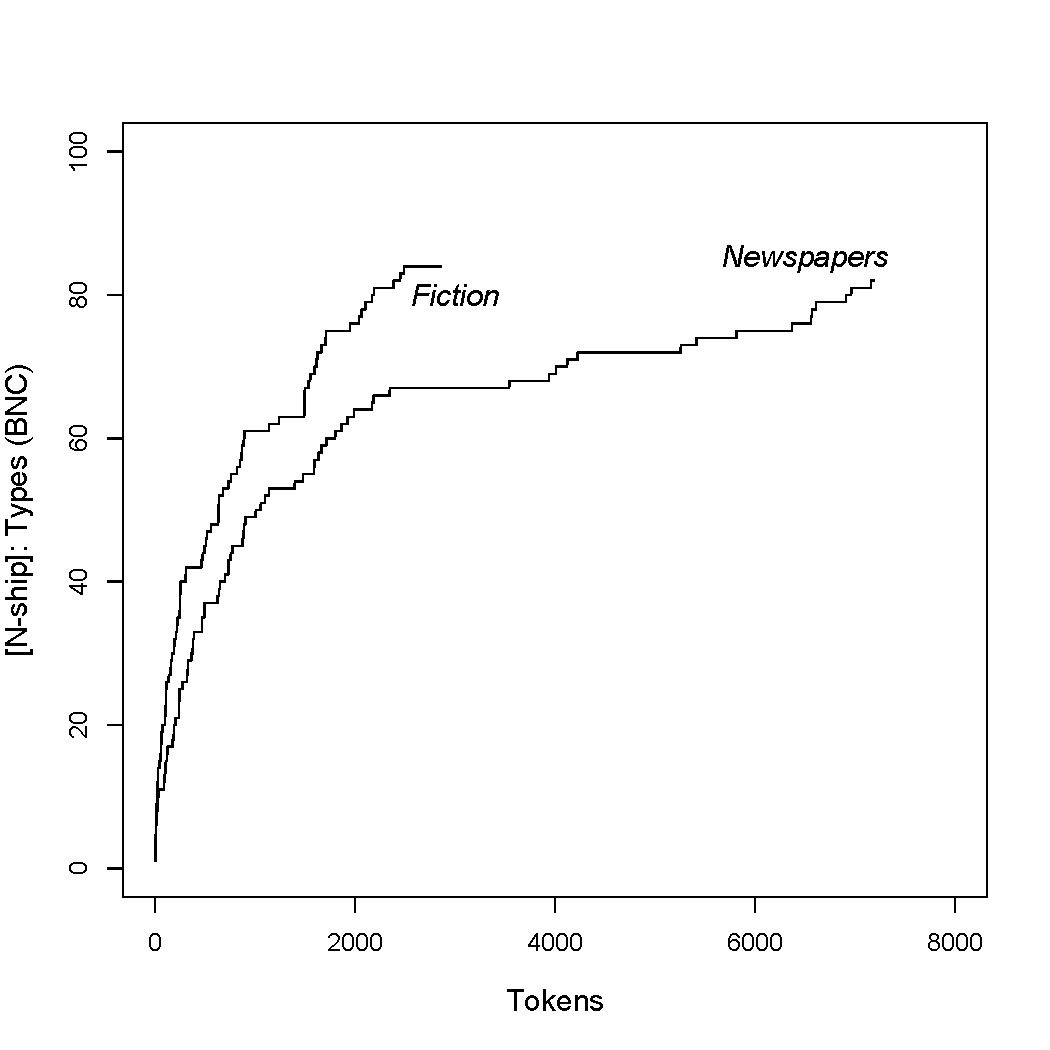
\includegraphics[width=.5\linewidth]{figures/genreshipfullttr}%
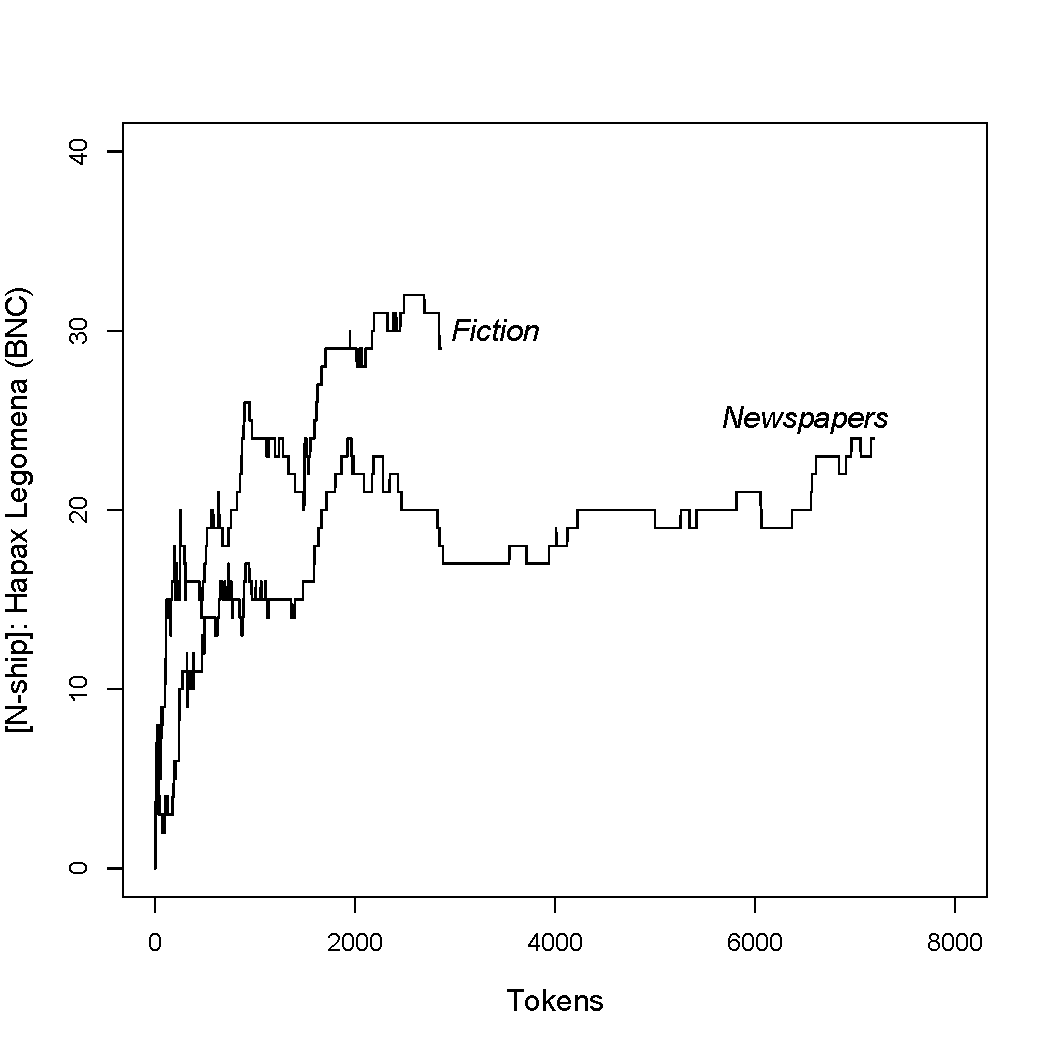
\includegraphics[width=.5\linewidth]{figures/genreshipfullhtr}%
\end{figure}

Both the TTR \is{type-token ratio} and the HTR \is{hapax-token ratio} suggest that the suffix \is{affix} is more productive \is{productivity} in fiction: \is{literary language} the ratios rise faster in \textvv{fiction} than in \textvv{newspapers} \is{newspaper language} and remain consistently higher as we go through the two sub\hyp{}corpora. It is only when the tokens have been exhausted in the fiction subcorpus but not in the newspaper subcorpus, that the ratios in the latter slowly catch up. This broadly supports our hypothesis, but let us look at the genre \is{genre} differences more closely both qualitatively \is{qualitative research} and \is{quantitative research} quantitatively.

In order to compare the two genres \is{genre} in terms of the type\hyp{}token \is{token (instance)}\is{type-token ratio} and hapax\hyp{}token \is{hapax-token ratio} ratios, they need to have the same size. \is{corpus size} The following discussion is based on the full data from the fiction \is{literary language} subcorpus and a subsample of the newspaper \is{newspaper language} corpus that was arrived at by deleting every second, then every third and finally every 192nd example, ensuring that the hits \is{hit} in the sample are spread through the entire newspaper \is{newspaper language} subcorpus.

Let us begin by looking at the types. \is{type (category)} Overall, there are 96 different types, 48 of which occur in both samples (some examples of types that frequent in both samples are \textit{relationship} (the most frequent word in the fiction sample), \textit{championship} (the most frequent word in the news sample), \textit{friendship}, \textit{partnership}, \textit{lordship}, \textit{ownership} and \textit{membership}. In addition, there are 36 types that occur only in the prose sample (for example, \textit{churchmanship}, \textit{dreamership}, \textit{librarianship} and \textit{swordsmanship}) and 12 that occur only in the newspaper sample (for example, \textit{associateship}, \textit{draughtsmanship}, \textit{trusteeship} and \textit{sportsmanship}). The number of types \is{type (category)} exclusive to each genre \is{genre} suggests that the suffix \is{affix} is more important in \textvv{fiction} \is{literary language} than in \is{newspaper language} \textvv{newspapers}.

The TTR \is{type-token ratio} of the suffix \is{affix} in newspaper language is $\nicefrac{60}{2862} = 0.021$, and the HTR \is{hapax-token ratio} is $\nicefrac{20}{2862} = 0.007$. In contrast, the TTR in fiction is $\nicefrac{84}{2862} = 0.0294$, and the HTR is $\nicefrac{29}{2862} = 0.0101$. Although the suffix, \is{affix} as expected, \is{frequency!expected} is generally not very productive, \is{productivity} it is more productive in fiction \is{literary language} than in newspapers. \is{newspaper language} As \tabref{tab:shipwords} shows, this difference is statistically significant in the sample ($\chi^2 = 4.1, \df = 1, p < 0.005$). This corroborates our hypothesis, but note that it does not tell us whether the higher productivity \is{productivity} of \textit{-ship} is something unique about this particular morpheme, \is{morphology} or whether fiction \is{literary language} generally has more derived words due to a higher overall lexical richness. To determine this, we would have to look at more than one \is{affix} affix.

\begin{table}
\caption{Types with \textit{-ship} in prose fiction and newspapers}
\label{tab:shipwords}
\begin{tabular}[t]{llccr}
\lsptoprule
 & & \multicolumn{2}{c}{\textvv{Type}} & \\\cmidrule(lr){3-4}
 & & \textvv{new} & \textvv{$\neg$new} & Total \\
\midrule
\textvv{\makecell[lt]{Genre}}
	& \textvv{fiction}
		& \makecell[t]{\num{84}\\\small{(\num{72.00})}}
		& \makecell[t]{\num{2778}\\\small{(\num{2790.00})}}
		& \makecell[t]{\num{2862}\\} \\
	& \textvv{newspaper}
		& \makecell[t]{\num{60}\\\small{(\num{72.00})}}
		& \makecell[t]{\num{2802}\\\small{(\num{2790.00})}}
		& \makecell[t]{\num{2862}\\} \\
\midrule
	& Total
		& \makecell[t]{\num{144}}
		& \makecell[t]{\num{5580}}
		& \makecell[t]{\num{5724}} \\
\lspbottomrule
\end{tabular}
\end{table}
% me: chisq.test(matrix(c(84,60,2778,2802),ncol=2),corr=FALSE)

Let us now turn to the hapax \is{hapax legomenon} legomena. These are so rare in both genres \is{genre} that the difference in TTR \is{type-token ratio} is not statistically significant, as \tabref{tab:shiphapaxes} shows ($\chi^2 = 1.67, \df = 1, p = 0.1966$). \is{chi-square test} We would need a larger \is{corpus size} corpus to see whether the difference would at some point become significant.

\begin{table}
\caption{Hapaxes with \textit{-ship} in prose fiction and newspapers}
\label{tab:shiphapaxes}
\begin{tabular}[t]{llccr}
\lsptoprule
 & & \multicolumn{2}{c}{\textvv{Type}} & \\\cmidrule(lr){3-4}
 & & \textvv{hapax} & \textvv{$\neg$hapax} & Total \\
\midrule
\textvv{\makecell[lt]{Genre}}
	& \textvv{fiction}
		& \makecell[t]{\num{29}\\\small{(\num{24.50})}}
		& \makecell[t]{\num{2833}\\\small{(\num{2837.50})}}
		& \makecell[t]{\num{2862}\\} \\
	& \textvv{newspaper}
		& \makecell[t]{\num{20}\\\small{(\num{24.50})}}
		& \makecell[t]{\num{2842}\\\small{(\num{2837.50})}}
		& \makecell[t]{\num{2862}\\} \\
\midrule
	& Total
		& \makecell[t]{\num{49}}
		& \makecell[t]{\num{5675}}
		& \makecell[t]{\num{5724}} \\
\lspbottomrule
\end{tabular}
\end{table}
% me: chisq.test(matrix(c(29,20,2833,2842),ncol=2),corr=FALSE)

To conclude this case study, let us look at a particular problem posed by the comparison of the same suffix \is{affix} in two genres \is{genre} with respect to the HTR. \is{hapax-token ratio} At first glance -- and this is what is shown in \tabref{tab:shiphapaxes} -- there seem to be 29 hapaxes \is{hapax legomenon} in fiction \is{literary language} and 20 in prose. However, there is some overlap: the words \textit{generalship}, \textit{headship}, \textit{managership}, \textit{ministership} and \textit{professorship} occur as hapax \is{hapax legomenon} legomena in both samples; other words that are hapaxes in one subsample occur several times in the other, such as \textit{brinkmanship}, which is a hapax in fiction but occurs twice in the newspaper sample, or \textit{acquaintanceship}, which is a hapax in the newspaper \is{newspaper language} sample but occurs 15 times in fiction.

It is not straightforwardly clear whether such cases should be treated as hapaxes. \is{hapax legomenon} If we think of the two samples as subsamples of the same corpus, it is very counterintuitive to do so. It might be more reasonable to count only those words as hapaxes whose frequency in the combined subsamples is still one. However, the notion ``hapax'' is only an operational \is{operationalization} definition for neologisms, \is{neologism} based on the hope that the number of hapaxes in a corpus (or sub\hyp{}corpus) is somehow indicative of the number of productive \is{productivity} coinages. We saw in Case Study \ref{sec:phonologicalconstraintsofify} that this is a somewhat vain hope, as the correlation \is{correlation} between neologisms and hapaxes \is{hapax legomenon} is not very impressive.

Still, if we want to use this operational \is{operationalization} definition, we have to stick with it and define hapaxes strictly relative to whatever (sub-)corpus we are dealing with. If we extend the criterion for hapax\hyp{}ship beyond one subsample to the other, why stop there? We might be even stricter and count only those words as hapaxes \is{hapax legomenon} that are still hapaxes when we take the entire BNC \is{BNC} into account. And if we take the entire BNC into account, we might as well count as hapaxes only those words that occur only once in all accessible archives of the language under investigation. This would mean that the hapaxes in any sample would overwhelmingly cease to be hapaxes -- the larger \is{corpus size} our corpus, the fewer hapaxes there will be. To illustrate this: just two words from the fiction \is{literary language} sample retain their status as hapax legomena if we search the Google Books collection: \textit{impress\hyp{}ship}, which does not occur at all (if we discount linguistic accounts which mention it, such as \citet{trips_lexical_2009}, or this book, once it becomes part of the Google Books archive), and \textit{cloudship}, which does occur, but only referring to water- or airborne vehicles. At the same time, the Google Books archive contains hundreds (if not thousands) of hapax \is{hapax legomenon} legomena that we never even notice (such as \textit{Johnship} `the state of being the individual referred to as \textit{John}'). The idea of using hapax legomena is, essentially, that a word like \textit{mageship}, which is a hapax in the fiction \is{literary language} sample, but not in the Google Books archive, somehow stands for a word like \textit{Johnship}, which is a true hapax in the English language.

This case study has demonstrated the potential of using the TTR \is{type-token ratio} and the HTR \is{hapax-token ratio} not as a means of assessing morphological \is{morphology} richness and productivity \is{productivity} as such, but as a means of assessing genres \is{genre} with respect to their richness and productivity. It has also demonstrated some of the problems of identifying hapax \is{hapax legomenon} legomena in the context of such cross\hyp{}variety \is{language variety} comparisons. As mentioned initially, there are not too many studies of this kind, but \citet{plag_morphological_1999} presents a study of productivity \is{productivity} across written \is{medium} and spoken language that is a good starting point for anyone wanting to fill this gap.

\subsubsection{Case study: Productivity and speaker sex}
\label{sec:productivityandspeakersex}

Morphological \is{morphology} productivity \is{productivity} has not traditionally been investigated from a sociolinguistic \is{sociolinguistics} perspective, but a study by \citet{saily_variation_2011} suggests that this may be a promising field of research. S\"{a}ily investigates differences in the productivity of the suffixes \is{affix} \textit{-ness} and \textit{-ity} in the language produced by men and women in the BNC. \is{BNC} She finds no difference in productivity for \textit{-ness}, but a higher productivity \is{productivity} of \textit{-ity} in the language produced by men (cf. also \citealt{saily_comparing_2009} for a diachronic \is{diachrony} study with very similar results). She uses a sophisticated method involving the comparison of the suffixes' \is{affix} type \is{type (category)} and hapax \is{hapax legomenon} growth rates, but let us replicate \is{replicability} her study using the simple method used in the preceding case study, beginning with a comparison of type\hyp{}token \is{type-token ratio} ratios.

The BNC \is{BNC} contains substantially more speech and writing \is{medium} by male speakers than by female speakers, which is reflected in differences in the number of affix tokens \is{token (instance)} produced by men and women: for \textit{-ity}, there are \num{2562} tokens produced by women and \num{8916} tokens produced by men; for \textit{-ness}, there are 616 tokens produced by women and \num{1154} tokens produced by men (note that unlike S\"{a}ily, I excluded the words \textit{business} and \textit{witness}, since they did not seem to me to be synchronically transparent instances of the affix). \is{affix} To get samples of equal size \is{corpus size} for each affix, \is{affix} random subsamples were drawn from the tokens \is{token (instance)} produced by men.

Based on these subsamples, the type\hyp{}token \is{type-token ratio} ratios for \textit{-ity} are 0.0652 for men and 0.0777 for women; as \tabref{tab:itysex} shows, this difference is not statistically significant ($\chi^2 = 3.01, \df = 1, p < 0.05, \phi = 0.0242$).\is{chi-square test}

\begin{table}
\caption{Types with \textit{-ity} in male and female speech (BNC)}
\label{tab:itysex}
\begin{tabular}[t]{llccr}
\lsptoprule
 & & \multicolumn{2}{c}{\textvv{Type}} & \\\cmidrule(lr){3-4}
 & & \textvv{new} & \textvv{seen before} & Total \\
\midrule
\textvv{\makecell[lt]{Speaker Sex}}
	& \textvv{female}
		& \makecell[t]{\num{167}\\\small{(\num{183.00})}}
		& \makecell[t]{\num{2395}\\\small{(\num{2379.00})}}
		& \makecell[t]{\num{2562}\\} \\
	& \textvv{male}
		& \makecell[t]{\num{199}\\\small{(\num{183.00})}}
		& \makecell[t]{\num{2363}\\\small{(\num{2379.00})}}
		& \makecell[t]{\num{2562}\\} \\
\midrule
	& Total
		& \makecell[t]{\num{366}}
		& \makecell[t]{\num{4758}}
		& \makecell[t]{\num{5124}} \\
\lspbottomrule
\end{tabular}
\end{table}

The type\hyp{}token \is{type-token ratio} ratios for \textit{-ness} are much higher, namely 0.1981 for women and 0.2597 for men. As \tabref{tab:nesssex} shows, the difference is statistically significant, although the effect size \is{effect size} is weak ($\chi^2 = 5.37, \df = 1, p < 0.05, \phi = 0.066$).

\begin{table}
\caption{Types with \textit{-ness} in male and female speech (BNC)}
\label{tab:nesssex}
\begin{tabular}[t]{llccr}
\lsptoprule
 & & \multicolumn{2}{c}{\textvv{Type}} & \\\cmidrule(lr){3-4}
 & & \textvv{new} & \textvv{seen before} & Total \\
\midrule
\textvv{\makecell[lt]{Speaker Sex}}
	& \textvv{female}
		& \makecell[t]{\num{122}\\\small{(\num{139.00})}}
		& \makecell[t]{\num{494}\\\small{(\num{477.00})}}
		& \makecell[t]{\num{616}\\} \\
	& \textvv{male}
		& \makecell[t]{\num{156}\\\small{(\num{139.00})}}
		& \makecell[t]{\num{460}\\\small{(\num{477.00})}}
		& \makecell[t]{\num{616}\\} \\
\midrule
	& Total
		& \makecell[t]{\num{278}}
		& \makecell[t]{\num{954}}
		& \makecell[t]{\num{1232}} \\
\lspbottomrule
\end{tabular}
\end{table}
% me: chisq.test(matrix(c(122,156,494,460),ncol=2),corr=FALSE)

Note that S\"{a}ily investigates spoken \is{medium} and written language separately and she also includes social class in her analysis, so her results differ from the ones presented here; she finds a significantly lower HTR \is{hapax-token ratio} for \textit{-ness} in lower\hyp{}class women's speech in the spoken subcorpus, but not in the written one, and a significantly lower HTR for \textit{-ity} in both subcorpora. This might be due to the different methods used, or to the fact that I excluded \textit{business}, which is disproportionally frequent in male speech and writing in the BNC \is{BNC} and would thus reduce the diversity in the male sample substantially. However, the type\hyp{}based \is{type (category)} differences do not have a very impressive effect size \is{effect size} in our design \is{research design} and they are unstable across conditions in S\"{a}ily's, so perhaps they are simply not very substantial.

Let us turn to the HTR \is{hapax-token ratio} next. As before, we are defining what counts as a hapax \is{hapax legomenon} legomenon not with reference to the individual subsamples of male and female speech, but with respect to the combined sample. \tabref{tab:ityhapaxsexlist} shows the hapaxes for \textit{-ity} in the male and female samples. The HTRs are very low, suggesting that \textit{-ity} is not a very productive \is{productivity} suffix: \is{affix} 0.0099 in female speech and 0.016 in male speech.

\begin{table}
\caption{Hapaxes with \textit{-ity} in sampes of male and female speech (BNC)}
\label{tab:ityhapaxsexlist}
\resizebox{0.9\textwidth}{!}{%
\begin{tabular}[t]{l}
\lsptoprule
\textvv{male speech} \\
\midrule
\makecell[tl]{
\begin{minipage}[t]{\textwidth} \raggedright
\textit{abnormality}, \textit{antiquity}, \textit{applicability}, \textit{brutality}, \textit{civility}, \textit{criminality}, \textit{deliverability}, \textit{divinity}, \textit{duplicity}, \textit{eccentricity}, \textit{eventuality}, \textit{falsity}, \textit{femininity}, \textit{fixity}, \textit{frivolity}, \textit{illegality}, \textit{impurity}, \textit{inexorability}, \textit{infallibility}, \textit{infirmity}, \textit{levity}, \textit{longevity}, \textit{mediocrity}, \textit{obesity}, \textit{perversity}, \textit{predictability}, \textit{rationality}, \textit{regularity}, \textit{reliability}, \textit{scarcity}, \textit{seniority}, \textit{serendipity}, \textit{solidity}, \textit{subsidiarity}, \textit{susceptibility}, \textit{tangibility}, \textit{verity}, \textit{versatility}, \textit{virtuality}, \textit{vitality}, \textit{voracity}
\end{minipage}} \\
\midrule
\textvv{female speech} \\
\midrule
\makecell[tl]{
\begin{minipage}[t]{\textwidth} \raggedright
\textit{absurdity}, \textit{adjustability}, \textit{admissibility}, \textit{centrality}, \textit{complicity}, \textit{effemininity}, \textit{enormity}, \textit{exclusivity}, \textit{gratuity}, \textit{hilarity}, \textit{humility}, \textit{impunity}, \textit{inquisity}, \textit{morbidity}, \textit{municipality}, \textit{originality}, \textit{progility}, \textit{respectability}, \textit{sanity}, \textit{scaleability}, \textit{sincerity}, \textit{spontaneity}, \textit{sterility}, \textit{totality}, \textit{virginity}
\end{minipage}} \\
\lspbottomrule
\end{tabular}}
\end{table}

Although the difference in HTR \is{hapax-token ratio} is relatively small, \tabref{tab:ityhapaxfrequencies} shows that it is statistically significant, albeit again with a very weak effect size \is{effect size} ($\chi^2 = 3.93, \df = 1, p < 0.05, \phi = 0.0277$).

\begin{table}
\caption{Hapax legomena with \textit{-ity} in male and female speech (BNC)}
\label{tab:ityhapaxfrequencies}
\begin{tabular}[t]{llccr}
\lsptoprule
 & & \multicolumn{2}{c}{\textvv{Type}} & \\\cmidrule(lr){3-4}
 & & \textvv{hapax} & \textvv{$\neg$hapax} & Total \\
\midrule
\textvv{\makecell[lt]{Speaker Sex}}
	& \textvv{female}
		& \makecell[t]{\num{25}\\\small{(\num{33.00})}}
		& \makecell[t]{\num{2537}\\\small{(\num{2529.00})}}
		& \makecell[t]{\num{2562}\\} \\
	& \textvv{male}
		& \makecell[t]{\num{41}\\\small{(\num{33.00})}}
		& \makecell[t]{\num{2521}\\\small{(\num{2529.00})}}
		& \makecell[t]{\num{2562}\\} \\
\midrule
	& Total
		& \makecell[t]{\num{66}}
		& \makecell[t]{\num{5058}}
		& \makecell[t]{\num{5124}} \\
\lspbottomrule
\end{tabular}
\end{table}
% me: chisq.test(matrix(c(25,41,2537,2521),ncol=2),corr=FALSE)

\tabref{tab:nesssexlist} shows the hapaxes for \textit{-ness} in the male and female samples. The HTRs \is{hapax-token ratio} are low, but much higher than for \textit{-ity}, 0.0795 for women and 0.1023 for men.

\begin{table}
\caption{Hapaxes with \textit{-ness} in samples of male and female speech (BNC)}
\label{tab:nesssexlist}
\resizebox*{0.9\textwidth}{!}{%
\begin{tabular}[t]{l}
\lsptoprule
\textvv{male speech} \\
\midrule
\makecell[tl]{
\begin{minipage}[t]{\textwidth} \raggedright
\textit{abjectness}, \textit{adroitness}, \textit{aloneness}, \textit{anxiousness}, \textit{awfulness}, \textit{barrenness}, \textit{blackness}, \textit{blandness}, \textit{bluntness}, \textit{carefulness}, \textit{centredness}, \textit{cleansiness}, \textit{clearness}, \textit{cowardliness}, \textit{crispness}, \textit{delightfulness}, \textit{differentness}, \textit{dizziness}, \textit{drowsiness}, \textit{dullness}, \textit{eyewitnesses}, \textit{fondness}, \textit{fulfilness}, \textit{genuineness}, \textit{godliness}, \textit{graciousness}, \textit{headedness}, \textit{heartlessness}, \textit{heinousness}, \textit{keenness}, \textit{lateness}, \textit{likeliness}, \textit{limitedness}, \textit{loudness}, \textit{mentalness}, \textit{messiness}, \textit{narrowness}, \textit{nearness}, \textit{neighbourliness}, \textit{niceness}, \textit{numbness}, \textit{pettiness}, \textit{pleasantness}, \textit{plumpness}, \textit{positiveness}, \textit{quickness}, \textit{reasonableness}, \textit{rightness}, \textit{riseness}, \textit{rudeness}, \textit{sameness}, \textit{sameyness}, \textit{separateness}, \textit{shortness}, \textit{smugness}, \textit{softness}, \textit{soreness}, \textit{springiness}, \textit{steadiness}, \textit{stubbornness}, \textit{timorousness}, \textit{toughness}, \textit{uxoriousness}
\end{minipage}} \\
\midrule
\textvv{female speech} \\
\midrule
\makecell[tl]{
\begin{minipage}[t]{\textwidth} \raggedright
\textit{ancientness}, \textit{appropriateness}, \textit{badness}, \textit{bolshiness}, \textit{chasifness}, \textit{childishness}, \textit{chubbiness}, \textit{clumsiness}, \textit{conciseness}, \textit{eagerness}, \textit{easiness}, \textit{faithfulness}, \textit{falseness}, \textit{feverishness}, \textit{fizziness}, \textit{freshness}, \textit{ghostliness}, \textit{greyness}, \textit{grossness}, \textit{grotesqueness}, \textit{heaviness}, \textit{laziness}, \textit{likeness}, \textit{mysteriousness}, \textit{nastiness}, \textit{outspokenness}, \textit{pinkness}, \textit{plainness}, \textit{politeness}, \textit{prettiness}, \textit{priggishness}, \textit{primness}, \textit{randomness}, \textit{responsiveness}, \textit{scratchiness}, \textit{sloppiness}, \textit{smoothness}, \textit{stiffness}, \textit{stretchiness}, \textit{tenderness}, \textit{tightness}, \textit{timelessness}, \textit{timidness}, \textit{ugliness}, \textit{uncomfortableness}, \textit{unpredictableness}, \textit{untidiness}, \textit{wetness}, \textit{zombieness}
\end{minipage}} \\
\lspbottomrule
\end{tabular}}
\end{table}

As \tabref{tab:nesssexfrequencies} shows, the difference in HTRs \is{hapax-token ratio} is not statistically significant, and the effect size \is{effect size} would be very weak anyway ($\chi^2 = 1.93, \df = 1, p > 0.05, \phi = 0.0395$).

\begin{table}
\caption{Hapax legomena with \textit{-ness} in male and female speech (BNC)}
\label{tab:nesssexfrequencies}
\begin{tabular}[t]{llccr}
\lsptoprule
 & & \multicolumn{2}{c}{\textvv{Type}} & \\\cmidrule(lr){3-4}
 & & \textvv{hapax} & \textvv{$\neg$hapax} & Total \\
\midrule
\textvv{\makecell[lt]{Speaker Sex}}
	& \textvv{female}
		& \makecell[t]{\num{49}\\\small{(\num{56.00})}}
		& \makecell[t]{\num{567}\\\small{(\num{560.00})}}
		& \makecell[t]{\num{616}\\} \\
	& \textvv{male}
		& \makecell[t]{\num{63}\\\small{(\num{56.00})}}
		& \makecell[t]{\num{553}\\\small{(\num{560.00})}}
		& \makecell[t]{\num{616}\\} \\
\midrule
	& Total
		& \makecell[t]{\num{112}}
		& \makecell[t]{\num{1120}}
		& \makecell[t]{\num{1232}} \\
\lspbottomrule
\end{tabular}
\end{table}
% me: chisq.test(matrix(c(49,63,567,553),ncol=2),corr=FALSE)

In this case, the results correspond to S\"{a}ily's, who also finds a significant difference in productivity \is{productivity} for \textit{-ity}, but not for \textit{-ness}.

This case study was meant to demonstrate, once again, the method of comparing TTRs \is{type-token ratio} and HTRs \is{hapax-token ratio} based on samples of equal size. \is{corpus size} It was also meant to draw attention to the fact that morphological \is{morphology} productivity \is{productivity} may be an interesting area of research for variationist \is{variation} sociolinguistics; \is{sociolinguistics} however, it must be pointed out that it would be premature to conclude that men and women differ in their productive use of particular affixes; \is{affix} as S\"{a}ily herself points out, men and women are not only represented unevenly in quantitative \is{quantitative research} terms (with a much larger proportion of male language included in the BNC), \is{BNC} but also in qualitative terms (the language varieties \is{language variety} with which they are represented differ quite strikingly). Thus, this may actually be another case of different degrees of productivity \is{productivity} in different language varieties (which we investigated in the preceding case study).

